%% LyX 2.1.4 created this file.  For more info, see http://www.lyx.org/.
%% Do not edit unless you really know what you are doing.
\documentclass[english]{book}
\usepackage[T1]{fontenc}
\usepackage[utf8x]{inputenc}
\usepackage{geometry}
\geometry{verbose,tmargin=2cm,bmargin=2cm,lmargin=2cm,rmargin=2cm,headheight=2cm,headsep=2cm}
\usepackage{float}
\usepackage{amsmath}
\usepackage{amssymb}
\usepackage{graphicx}

\makeatletter

%%%%%%%%%%%%%%%%%%%%%%%%%%%%%% LyX specific LaTeX commands.
%% Because html converters don't know tabularnewline
\providecommand{\tabularnewline}{\\}
\floatstyle{ruled}
\newfloat{algorithm}{tbp}{loa}
\providecommand{\algorithmname}{Algorithm}
\floatname{algorithm}{\protect\algorithmname}

%%%%%%%%%%%%%%%%%%%%%%%%%%%%%% User specified LaTeX commands.
\usepackage{babel}

\usepackage{babel}

\makeatother

\usepackage{babel}
\begin{document}

\title{Modélisation, Simulation multi-niveau pour l'optimisation de politiques
de vaccination}


\author{TRAN Thi Cam Giang, Jean Daniel ZUCKER, Marc CHOISY, Yann CHEVALEYRE}


\date{03/06/2015}

\maketitle

\part{INTRODUCTION}


\section{Problematic}


\subsection{Current Status of Infectious Diseases }

According to the 2004 Global Burden of Disease report of the world
Health Organization, infectious disease is the leading cause of death
of children and adolescents, and one of the main causes in adults.
Infectious disease brings for six of the top 20 leading causes of
death worldwide. In low-income countries, infectious disease represents
six of the top 10 most common causes of death. This thesis is proposed
in the context when the world started struggling with a global recession
and in the same time, many public health serious events have occurred
in the world : SRAS in 2003, avian influenza in 2004 or swine flu
in 2009, etc. Besides, we had to face up to ``re-emerging'' infectious
diseases that were thought to be waning. For example, particularly
and quite surprisingly one of the vaccine-preventable diseases is
measles that returned backs in all the world and much stronger than
before. At the start of 2014, the World Health Organization (WHO)
officially stated global measles epidemic outbreak. In the first three
months of the year 2014, there were about 56,000 cases of measles
infections in 75 countries, particularly in southeast Asia and in
Vietnam. More specially, in the United States, measles cases significantly
rose in 2014, 14 years after national leaders stated that the disease
had been disappeared within the country. There were 288 cases of measles
reported in the U.S between Jan. 1 and May 23, 2014 as in figure \ref{fig:measlesUS20012014}.
To explain this sudden outbreak of the measles, epidemiologist found
out that the reasons are strongly relative to international travel
by unvaccinated people (particularly U.S. residents), and incomplete
vaccination that the American government doesn't control.

\begin{figure}[h]
\centering 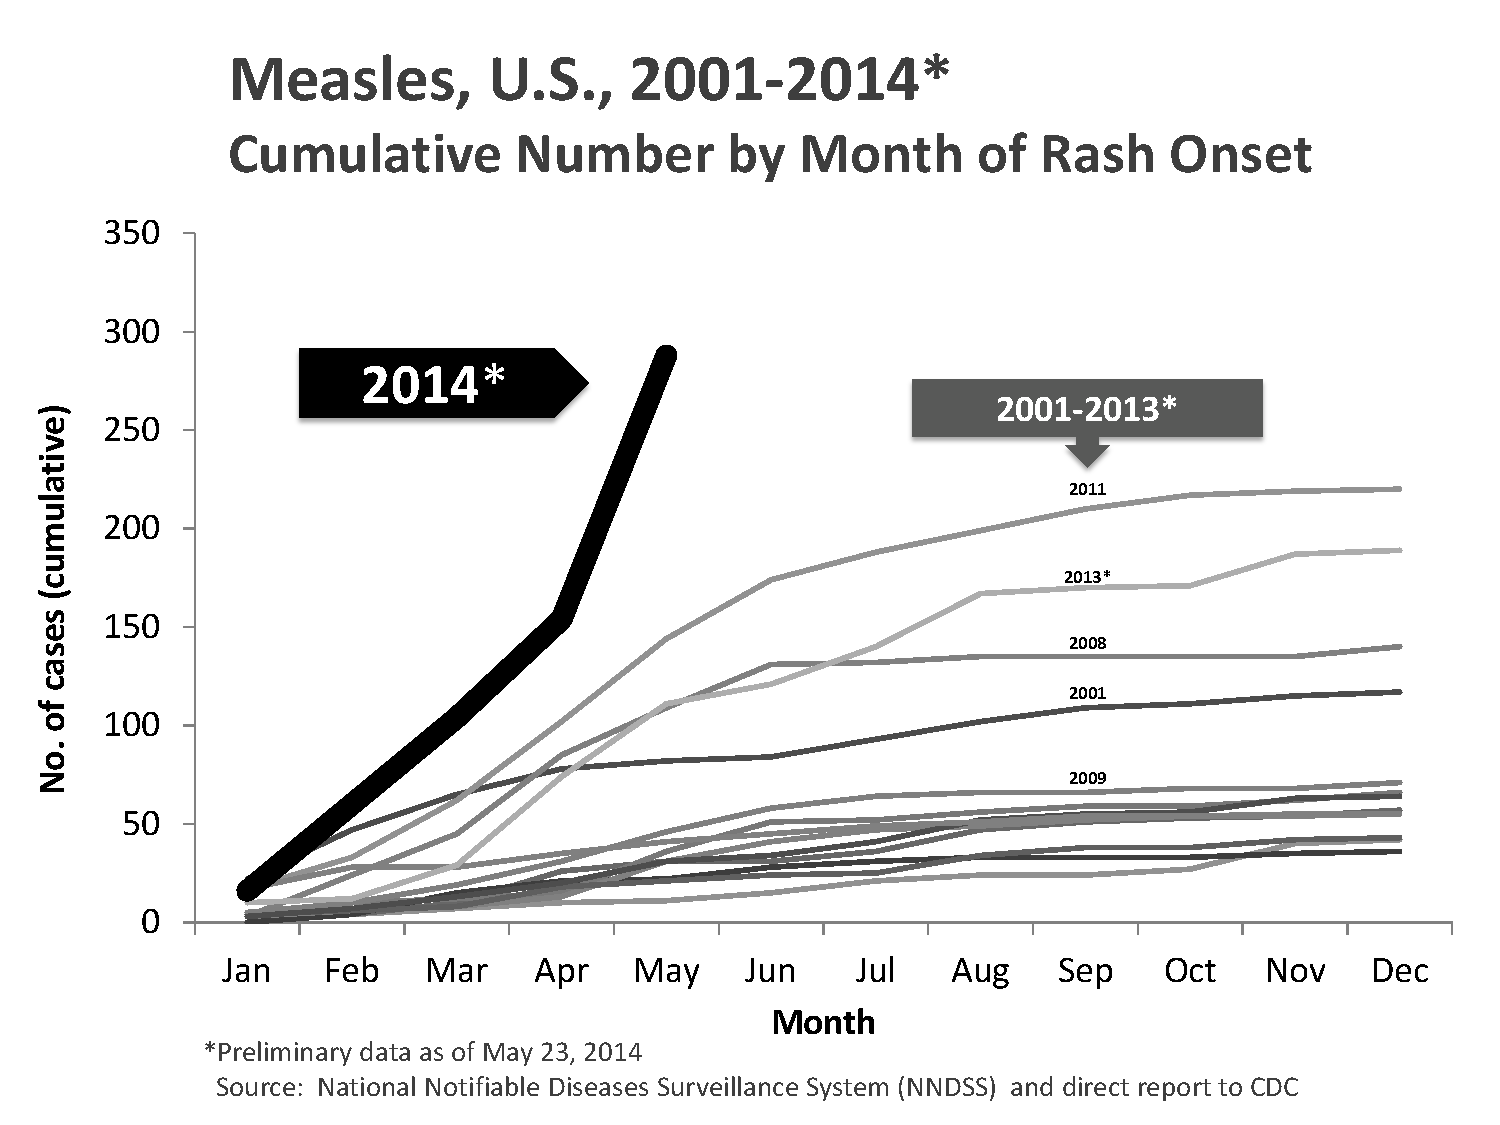
\includegraphics[scale=0.5]{/home/tran/Desktop/These_TTCGIANG/THESE_GitHub/Manuscrist/Manuscrit/shareLatex/version2/figure/measlesUS20012014}
\protect\caption{Measles, U.S., 2001-2014: Cumulative Number by Month of Rash Onset}
\label{fig:measlesUS20012014} 
\end{figure}


Moreover, the world has to face up new infectious diseases that were
once unknown or already known in past but totally to be waning, such
as Ebola epidemic, in the same year to the measles. The Ebola epidemic
is the largest in human history, affecting almost all countries in
West Africa. To date, the WHO have reported a total of 28,575 suspected
cases and 11,313 deaths. However, it is numbers in documents understated
for the magnitude of the outbreak. Now, in Liberia, the government
was officially stated Ebola-free in May 2015, however new cases were
found in late June and early July. The world suffered two large epidemics
in the same year, this has stressed the importance of the epidemiological
phenomena anticipation when diseases occur. Many studies proposed
by the WHO, the Pasteur Institute and the Inserm in the field of environmental
security have tried to understand disease phenomena and spread of
disease over a territory, to better manage when diseases occur. 

Hence, infectious diseases is becoming more complex, and more variant.
We are difficult to well control the spread of infectious diseases
even vaccine-preventable diseases as meals. 

With the current epidemic state of the world, the main reasons to
explain the reemergence of old communicable diseases and the emergence
of new ones as follows : 
\begin{itemize}
\item changes of environment where we live in : 

\begin{itemize}
\item (1) Increased movements of people, 
\item (2) expansion of international trade in foodstuffs and medicinal biological
products, 
\item (3) social and environmental changes linked to urbanization, 
\item (4) deforestation, 
\end{itemize}
\end{itemize}
These four reasons change rapidly the nature of the world where we
live in, but our human is not becoming to. However, the main agents
of infectious diseases such as bacterial, fungal, parasitic, and viral
already rapidly adapt to new environment. 

Evolution of drugs that is used for the curative treatments of infectious
disease, have become less effective and developed less slowly than
the adaption of parasites. 

Hence, we are preceding two great challenges : 
\begin{itemize}
\item we keep on promoting the evolution of antimicrobial resistance for
infectious disease. 
\item It is necessary to understand the environmental factors that contribute
to the emergence and re-emergence of infectious diseases and the process
of disease spread to develop tools that will enable detecting and
monitoring of how diseases spread, so that they can be identified
and controlled before these infectious disease become pandemics.
\end{itemize}
Because the evolution of drugs is always slower than the adaption
of parasites in environmental changes, thus now we focus on tools
that will enable detecting and predicting diseases spread before they
become pandemics. 


\subsection{Disease Control Policy}

Pathogenic microorganisms such as bacteria, viruses, parasites or
fungi are key factors causing infectious diseases. The diseases can
be spread directly or indirectly from one person to another, through
a mediate environment or contaminated tools. As far as directly infectious
diseases are concerned, meaning diseases directly transmitted from
one person to another, we have some normal policies to prevent the
spread of diseases such as vaccines, anti-viral medications, and quarantine. 

\textbf{A. Quarantine: }

Quarantine is a policy to protect the public of disease by separating
and restricting the movement of people in community who have or may
have a contagious disease. 
\begin{itemize}
\item \textbf{Advantages: }

\begin{itemize}
\item Quarantine can be applied to humans as well as animals to protect
the spread of disease. 
\item Quarantine simply is a precautionary measure that breaks the line
of transmission from infected individuals to others. This method allows
health authorities to prevent further spread of a disease in the case
the quarantined individual develops clinical symptoms of the disease
of concern. 
\end{itemize}
\item Disadvantages: 

\begin{itemize}
\item The main method of the quarantine is to separate and restrict the
movement of people in community. This method really is effective in
a public health to prevent spread of a disease. However it has to
face adverse consequences for civil liberties (ethical and human rights)
and economic status (border closures and travel restrictions). Big
challenge is proposed how we can guarantee tradeoffs between personal
freedom and public good in preparing for a pandemic. $\backslash$cite\{choffnes2007ethical\} 
\item In the case, disease has a long incubation period and do not have
highly evident symptoms. Everything needs to be checked for suspected
cases, so can be quite time consuming. 
\item Quarantine is only effective as a PHYSICAL barrier to disease. Hence,
it is not effective for disease of animal, particularly wild birds.
\end{itemize}
\end{itemize}


\textbf{B. Anti-viral medications: }

Antiviral medications usually are called drugs used specifically for
treating viral infections. Antiviral drugs are medicines in form (pills,
liquid, an inhaled powder, or an intravenous solution) that makes
the ability of viruses decrease to reproduce. So, these drugs may
help reduce the duration of symptoms caused by virus. 
\begin{itemize}
\item Advantages : 

\begin{itemize}
\item Antiviral drugs are recommended for both treatment and prevention
of virus replication. For example, for influenza, within 48 hours
of onset of flu symptoms, antiviral drugs work best, but they may
still offer benefits when taken later. These medications may reduce
the duration of flu by one to two days and prevent severe flu complications.
Moreover, when you get the flu, the antiviral drugs is a best choose. 
\item Current antiviral drugs now are designed to help deal with HIV, herpes,
viruses, the hepatitis b and C viruses, and influenza A and B viruses.
\end{itemize}
\item Disadvantages: 

\begin{itemize}
\item Designing safe and effective antiviral drugs is difficult, because
viruses use the host's cells to replicate. 
\item Antiviral drugs sometimes are serious, particularly for children and
newborn babies. It is necessary to speak with doctor before making
any decisions about medications. 
\item Antiviral drugs only work best within when taken within 48 hours of
onset of flu symptoms. It is not good to prevent diseases before taking
diseases. For some diseases that have vaccines, antiviral drugs are
a second method of defense to treat diseases if you get it. Vaccines
are still the first and best way to prevent diseases.
\end{itemize}
\end{itemize}


\textbf{C. Vaccination: }

A vaccine is understood as a biological preparation that provides
active acquired immunity to a particular disease for our body. After
having been vaccinated, we transport microorganisms in weakened or
killed form of the microbe into our body. The body's immune system
produces the right antibodies to recognize the germs as a threat,
destroy them and keep a record of them. Because of that, when the
disease occurs, our immune system can recognize and destroy with a
better chance of success any of these germs that it later encounters.
In past, vaccination has greatly helped human beings. The vaccination
of influenza, Human Papillomavirus (HPV) and chicken pox have been
particularly appreciated. Smallpox is a particular example. It was
a big black point in human history during the closing years of the
18th century. Smallpox killed an estimated 400,000 Europeans annually
and among the people that luckily survived, a third had been blinded
by the disease. However, the WHO officially stated the eradication
of smallpox in 2011 $\backslash$cite\{tognotti2010SmallpoxErad,fenner2001SmallpoxErad\}.
Many infectious diseases are clearly restricted such as influenza,
polio, measles and tetanus from much of the world. 
\begin{itemize}
\item Advantages: 

\begin{itemize}
\item The biggest benefit of vaccine is individual immunity: It provides
long-term, sometimes lifelong protection against a disease. The vaccines
recommended in the early childhood immunization schedule protect children
from common infectious diseases worldwide (measles, chicken pox and
other illnesses). As children grow older, additional vaccines protect
them from diseases that affect adolescents and adults, as well as
for diseases they may encounter during travel to other regions. 
\item The secondary benefit of vaccination, is herd immunity (or called
also community immunity). When vaccination rates in a community is
high, so herd immunity can protect people who are unable to receive
vaccinations (including newborns and individuals with chronic illnesses)
from diseases. Hence, it is difficult for the disease to gain an outbreak
in the community. Vaccination has greatly reduced the burden of infectious
diseases. 
\item Vaccination is different from giving medicine to an unwell child to
make them better. The benefits of vaccination are invisible. 
\end{itemize}
\item Disadvantages: 

\begin{itemize}
\item The ability of disease outbreak strongly depends on community vaccination
rates. Widespread disease outbreaks can occur if the vaccination rates
drop below the threshold of herd immunity. Thus, the problem about
the vaccination rates is a big problem for countries that have complex
geographic system. 
\item Deciding not to vaccinate children puts them at risk of catching a
range of potentially serious, even fatal, diseases. 
\item Expensive. 
\end{itemize}
\end{itemize}


In short, we find that among three policies to prevent spread of diseases,
the vaccination policies bring more benefits than two methods left.
The vaccination policies build a complete immune system against diseases
for children in long-term or lifelong. Moreover, vaccines can prevent
spread of disease in an entire community. Due to two strong benefits,
the vaccination programmes have been deployed in the world. However,
according to the U.S. childhood vaccination schedule for children
between birth and six years, 14 different diseases are recommended
for immunizations. 14 base vaccines must vaccinate children in an
obligatory age is a very difficult financial problem for governments
as well as parents in low-income countries. To solve the financial
problem and at the same time to prevent the disease outbreak in the
world, WHO always try to provide more free vaccines for poor countries.
But nowadays, no infectious disease is completely eradicated. 

One question is posed why the human is still facing up to infectious
diseases when most of common infectious disease have vaccines. It
is obvious that the thorough knowledge of the disease is essential
in order to implement large-scale proper infection control measures
and prevention campaigns. The disease transmission methods depend
on the characteristics of each disease and the nature of the microorganism
that causes it. However, as mentioned above, vaccination rates strongly
influences the ability of disease outbreak in the community. If in
a community, the rate of vaccinated individuals is more than 80\%,
so this community is completely protected from a disease. But, in
fact, it is very rare to have a community of 80\% vaccinated individuals,
and more rarely in pour countries. 

Our current mass policy (for example the routine measles vaccination
policy for measles) that vaccinates the maximum number of children
before a certain age, is the oldest (started from the 1950s in the
rich countries) and is now the most used. The policy has obtained
main result that is a clear decrease of the incidence in most countries.
However, due to the nature of this mass policy, the problem of this
vaccination policy is too expensive, really ineffective and quite
impossible to implement in poor countries, especially in Africa because
of both financial and logistical problems. (e.g. the WHO project \textquotedbl{}Extended
Program on Immunization\textquotedbl{} in Vietnam for the measles
extinction before 2012 failed). 

Hence, the challenge is posed that there is a way that can help us
predict the effective of a vaccination policy before we place it.
Because, in fact when a vaccination policy is performed in a country,
there is only one policy deployed. One single policy is placed in
a community and after a couple of years we can start evaluating the
effective of the policy. This is very expensive and loses time. 

Need a tool new optimal vaccination policies in artificial intelligence
in order that these policies may become more effective, less expensive,
and take into account the spatial dimension for all popular infectious
diseases. Modeling tools are proposed to simulate disease transmission
dynamics of vaccine-preventable diseases and to investigate and predict
the effect of vaccination policies on the spread of diseases in the
entire world. 


\subsection{Current Modeling Tools }

As we know, increased movements of people world-wide is the leading
factor of the ability of spread of infectious disease. Recent works
have shown that infectious diseases can spread and outbreak in space
{[}9, 15, 35, 37{]}. There are many factors that affect the spread
in space such as: local factors (demographic including population
size {[}19{]}, growth rate and death rate {[}7{]}, sociological such
as school period of children, work tendency from rural to urban, environmental
and climatic comprising seasonal variations in seasonality {[}8, 17{]},
temperature and rainfall, immunological for diseases, etc...), and
global factors (the connections between the different populations
(i.e. spatial structure) {[}40{]} such as distance {[}19{]}, coupling
rate, number of individuals between populations, etc....). Hence,
knowledge of these factors is very difficult, but extremely essential
to inform models and computational efforts. It is the reason why there
are few empirical studies available that provide estimates of the
number and duration of contacts between subpopulations in a metapopulation.
Moreover, the role of the infectious disease modeling has a big signification
for us. For examples, due to these, we can simulate the spread of
infectious diseases in subpopulations, the interaction among subpopulations.
We can observe and understand the emergent dynamics of epidemics.
Then, we can predict and anticipate the scales of infectious disease
dynamics. Thus, we can give proper policies to minimize the infected
number and better manage when diseases occur. Hence, there are already
some packages in R that support us doing simulations, such as : ``adaptivetau'',
``GillespieSSA'' and ``EpiDynamics''. These packages allow us
to simulate dynamics of epidemics. However, they have many disadvantages:
(1) simulation in R is naturally slow, (2) these packages don't perform
modeling for a meta-population of many subpopulations, so simulating
the dynamics of a meta-population is very difficult, and the time
to implement simulations is very big, (3) R uses virtual memory to
hold objects, this causes design limitations on great objects, hence
users see always issues in R memory, specially anyone who works with
large datasets. 

Therefore, challenge to us is to create a tool that permits us to
model infectious disease dynamics in a metapopulation, to hurry up
simulations, and become a useful tool to support decision of public
healthy policies used by health professionals. 


\section{Motivation of thesis}

This thesis is proposed in epidemic context where many infectious
diseases such as measles, dengue in Asia and most countries of southeast
Asia are more and more seriously occurring in incidence and geographic
range; and there are emerging infectious diseases such as Ebola, Zika.
Besides, the mass policy, the oldest and still most widely used in
the world, is to vaccinate a maximal number of children before a certain
age. This policy is already obtaining a significant decrease about
the incidence in many countries. However, it is too expensive, ineffective
and absolutely impossible to implement in many poor and low-income
countries, in particular in Africa, Southeast Asia because of financial
and logistical problems. On the other hand, the number of the tool
supporting prediction of disease spread is still limited. Hence, there
are many challenges pointed to this thesis. The first urgent request
is to propose an efficient algorithm for optimizing vaccination policies
evaluated by spacial and stochastic simulation. More urgently, we
must have an informatics tool supporting decision of vaccination policies
used by health professionals available in the form of an R package
that can integrate R and C++ to speed up simulations. 

In this thesis, we will focus on modeling of popular infectious diseases
with transmission by direct contact. This transmission requires a
close contact between an infected person and a susceptible person,
such as touching an infected individual, kissing, sexual contact with
oral saliva, or contact with body lesions. These diseases usually
occur between members of the same household or close friends and family.
In particular, this thesis will mostly focus on measles. Measles is
a highly contagious, serious disease caused by a virus. It is a typical
infectious disease with direct transmission. In 1980, approximate
$2.6$ million people was killed each year before we had the widespread
vaccination policies. It spreads very fast by coughing and sneezing
in human communities via close interpersonal contact or direct contact
with secretions. Its main symptoms consist of high fever, cough, runny
nose and red eyes. These first symptoms usually take from $10$ to
$12$ days after exposure to an infectious person, and lasts $4$
to $7$ days \cite{panum1988observations}. Nowadays, there is no
proper treatment for measles to totally prevent the spread of measles
except routine measles vaccination policy for children. According
to the report by the WHO, since 2002 measles was eradicated from U.S.
However, today measles vaccination has not been extensively popularized
in the entire world. Beside the obtained results, for example, in
2013, there was about 84$\backslash$\% of the world's children having
received one dose of measles vaccine, and during 2000-2013, measles
vaccination prevented an estimated 15.6 million deaths; we have had
to face up about 145700 measles deaths globally-estimated 400 deaths
every day or 16 deaths every hour in 2013. Measles becomes one of
the leading causes of death among young children in the world, although
now we are having a big stock of safe and readily available measles
vaccines. 

In short, build a tool to optimize vaccination policies in order that
these policies may become more effective, less expensive, and take
into account the spatial dimension for all popular infectious diseases,
in particular fir measles.\pagebreak{}


\part{STATE OF THE ART}


\section{Model}


\subsection{Spatial structures for metapopulation model }

For directly transmitted infectious diseases by virus and bacteria,
susceptible individuals are not only infected by infected individuals
in the same location, but also by other infected individuals due to
the movement of individuals between populated regions. This is one
very important part in the domain studying the geographical spread
of infectious diseases. We care for host population characteristics,
then characteristics of spatial spread of an infectious disease among
populations. Through these characteristics, we find optimal policies
to minimize the number of infected individuals in a community. In
fact, there are many studies about the interactions among populations.
However, we can divide the spatial structure of populations into two
main levels: \textquotedbl{}inter-city level\textquotedbl{} and \textquotedbl{}intra-city
level\textquotedbl{}. At the inter-city level (or called \textquotedbl{}micro-level\textquotedbl{}),
we use differential equations to control its models. At the \textquotedbl{}intra-city
level\textquotedbl{} ( also called \textquotedbl{}macro-level\textquotedbl{})
in which we provide connections between the populations, simulate
the intra-city traffic. We consider the effect of travel through the
connections between population regions as a means of spreading a virus
\cite{shaw2010effective}. Focusing on the \textquotedbl{}macro-level\textquotedbl{},
we have two basic models considered : (1) the model has no explicit
movement of individuals and (2) the models describes enough travels
and movements of individuals among populations and even takes into
account the resident population as well as the current population
of individuals \cite{van2008spatial}. 
\begin{enumerate}
\item The spatially-nonexplicit model


A population may be simplified as a city, community, or some other
geographical region. Population travel (e.g. among animals and among
people by foot, birds, mosquitoes and in particular, people travel
by air from one city to another), is the main reason why diseases
can spread quickly among very distant cities such as SARS disease
in 2003. Therefore, the term \textquotedbl{}metapopulation\textquotedbl{}
arrived in the ecological literature in 1969 by Levins \cite{Levins1969,hanski1991metapopulation}.
A metapopulation is a population of a set of spatially discrete local
populations (or subpopulations in short) with mutual interaction \cite{Levins1969}.
In the metapopulation in which a subpopulation can only go extinct
locally and be recolonized by another after it is emptied by extinction
\cite{Bolker1996,Hanski1998,Levins1969} and migration between subpopulaitons
is significantly restricted. In a metapopulation, if recolonization
rates are smaller than extinction rates, then total extinction of
all local population will easily be reached. The persistence time
of the metapopulation is measured as the time until all subpopulations
go extinct. According to Harrison (1991) \cite{hanski1991metapopulation}
there are four types of spatially dynamic populations : classic Levins
metapopulation, mainland-island metapopualtion, patchy population
and non-equilibrium populations.
\begin{itemize}
\item \textbf{Classic Levins metapopulation:}
\end{itemize}

The first metapopulation model was proposed in 1969 by Levins. It
is called the classic Levins Metapopulation \cite{Levins1969}. Wilson
in 1980 \cite{wilson1980natural} stated that in this classic model
\textquotedbl{}A nexus of patches, each patch winking into life as
a population colonizes it, and winking out again as extinction occurs.''


\begin{figure}[h]
\centering 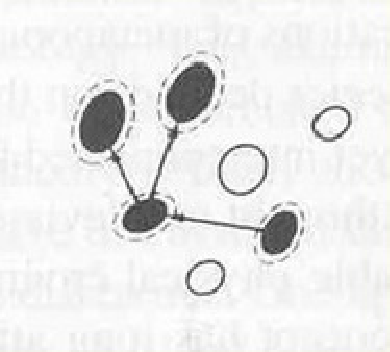
\includegraphics{figure/classicLevinsMeta} \protect\caption{Classic Levins Metapopulation Model \cite{harrison1997empirical}}
\end{figure}



All subpopulations in this classic model are relatively small. The
levels of interaction among individuals within a subpopulation is
much higher than between subpopulations.
\begin{itemize}
\item \textbf{Mainland-island metapopulation:}
\end{itemize}

The second model is the mainland-island metapopulation in which there
are some small \textquotedbl{}island\textquotedbl{} subpopulations
within dispersal distance of a much larger \textquotedbl{}mainland\textquotedbl{}
subpopulation.


\begin{figure}[h]
\centering 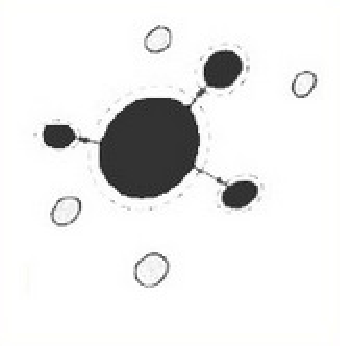
\includegraphics{figure/mainlandIslandMeta} \protect\caption{Mainland-Island Metapopulation \cite{harrison1997empirical}}
\end{figure}



It is evident that smaller sub-populations have a high probability
of local extinction, but the mainland population will hardly become
extinct. The migration from the mainland to the islands is independent
of the islands white or filled, but is propagated for the connected
islands. Therefore, if the mainland population has a low individual
density and there is no immigration, then population growth rate is
positive. Inversely, if island populations are in the same conditions
as the mainland, then its population growth rate is negative. Thus,
the islands would go down to extinction if there are no immigrants.
\begin{itemize}
\item \textbf{Patchy population:}
\end{itemize}

The third model is patchy population. The local populations exist
in a big habitat population and the dispersal rate between sub-populations
is high.


\begin{figure}[h]
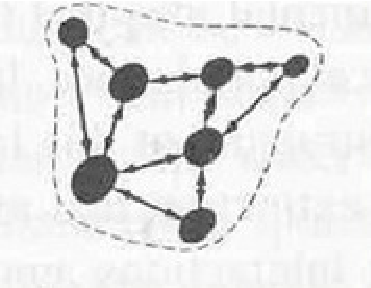
\includegraphics{figure/figPatchyPopulation} \protect\caption{Patchy population \cite{hanski1991metapopulation}}
\end{figure}



Here we can find that the population structure is grouped and the
interaction among them is frequent. However, this model is not referred
as a concept for metapopulation and most researchers do not consider
this a meta-population either.
\begin{itemize}
\item \textbf{Non-equilibrium populations:}
\end{itemize}

The final model is the non-equilibrium population. The local populations
are patches, its local extinctions are much greater than its recolonisation.


\begin{figure}[h]
\centering 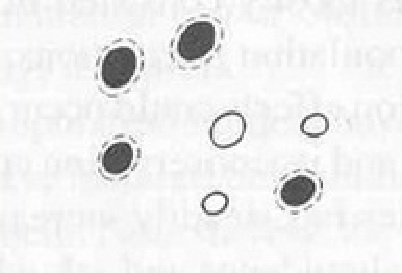
\includegraphics{figure/figNonEquilibriumPopulation}
\protect\caption{Non-equilibrium population \cite{hanski1991metapopulation}}
\end{figure}



It is obvious that white patches are rarely or never recolonized.
Therefore, this model is not considered as a functional metapopulation.
We can find this model in forested agricultural fields.


We already have four metapopulation models. In order to model the
metapopulations mentioned above, we have three main model to implement
: spatially-implicit model, spatially-explicit model and spatially-realistic
model. For the first model, this is the type of model used in Levins
(1969) \cite{Levins1969} in which supposing that all local populations
are connected with each other and they have independent local fluctuations.
At any one time, we save track of the proportion of local populations
and we do not take care the distance between them and the population
size of each subpopulation. This model are mathematically and conceptually
easy to implement. But this model can only answer some metapopulation
problems because it ignores so many variables of a metapopulation.
This model should be used for metapopulation close to a steady state.

\item The spatially-explicit model


For the second model, the spatially-explicit model is more complex
than the first model. Subpopulations may be filled or vacant. Local
populations only have interactions with the nearest neighbors. Subpopulations
are organized as cells on a grid and migration among them depends
on population density. We also only consider presence or absence of
a species in each subpopulation. The advantage of this model is easy
to model because of same local behaviors from subpopulation to subpopulation.
However, we cannot simply describe the state of the metapopulation
through filled subpopulations. Finally, the spatially-realistic model
uses GIS to realize attributes, geometric coordinates, etc ... to
a metapopulation. The first author using this model is Hanski in 1994
\cite{hanski1994practical}. His model was defined as the incidence
function (IF) model. This model is more realistic, and we can estimate
quantitative predictions about metapopulation fluctuation. However,
in fact, this model is very complicated, and many geographic data
have to be estimated. Hence, the metapopulation concept start to no
longer exist.

\end{enumerate}
In the scope of this thesis, we focus on a metapopulation model that
is result of combination between the spatially-explicit model and
the patchy population. In general, this a simple spatial model, but
is one of the most applicable model to descrire spread of diseases
in human communities. This metapopulation consists of distinct subpopulations,
each of which fluctuates independently, together with interaction
limited by a coupling parameter $\rho$. These subpopulations may
be filled or empty and contact with any neighbours.


\subsection{Epidemic models}

It is known that, there are many current models that are used to model
complex systems in nature, in ecology system and in epidemiology.
Mathematical models in epidemiology are a typical example. These models
permit us to present behavior of diseases and disease process in mathematics.
However, explaining the transmission of infectious diseases is a difficult
problem for an epidemiologist. Because there are many different interacting
factors causing the outbreak of diseases such as the environment,
the climate, the geography, the culture,...Hence, the role of the
epidemiologist is how to model the characteristics and the transmission
process of an infectious disease. Researchers have proposed compartmental
models in epidemiology by dividing the population into “compartments''
that illustrate health states of human through individuals. These
compartmental models are called the epidemic models too. The first
benefit of these models is to model the transmission process of a
communicable disease through compartments. Then, we can predict the
properties of the disease dynamics such as the estimated number of
infected individual, the time of persistence of disease, further that
where and when we can implement vaccination policies to have both
a minimum number of vaccined individuals and the minimum number of
infected individuals in a given population. Let image that now in
your country, there is an infectious disease as measles, a baby can
be infected. According to the process of infection of disease, firstly
this baby was born, he is fine and he is not infected yet by the measles
but he may be infected in the future. We say that he belongs to the
susceptible group (in short, S). Then, his mother takes him to a supermarket,
there he see so many people, he is really infected through any way.
He starts having a high fever, he may have to pass this state from
$3$ days to $5$ days. In this period, he is really infected but
he cannot infected others. We say that he belong to the exposed group
(in short, E). After that, he start decreasing the temperature, but
at the same time, he begins having red rashes on the back of the ears,
after a few hours, on the head, on the neck and finally most of the
body. This period appears from five to eight days after the exposed
step. This duration is very sensible. The baby is completely infected
and he can infected others if they see him. He belongs to the infected
group (in short, I). Finally, he passes to the final period, he comes
back good state. We say that he belongs to the recovered group with
immunity (in short, R).

Around these four main health groups presenting the process of infection
propagation in community, there are many epidemic models proposed.
We give here the development of epidemic models by focusing on acute
infections, assuming the pathogen causes illness for a periods of
time followed by (typically lifelong) immunity. The first simplest
model is the S-I-R model created by W. O. Kermack and A. G. McKendrick
in 1927. The authors categorized hosts within groups as described
above \textbf{S}usceptible (if not yet exposed to the pathogen), \textbf{I}nfected
(if currently infected by the pathogen) and \textbf{R}ecovered (if
they have successfully cleared the infection). From the simplest SIR
model, in order to accord each infectious disease and real property
of disease, scientists have modified it, made it different multiform.
However, in shape of this thesis, we concentrate on the SEIR model
(as the figure \ref{fig:seirmodel}) that fit many currently infectious
diseases in the world. Each patient must pass four health steps :
susceptible stage, incubation stage, infectious stage and recovered
stage.

\begin{figure}[tbph]
\centering 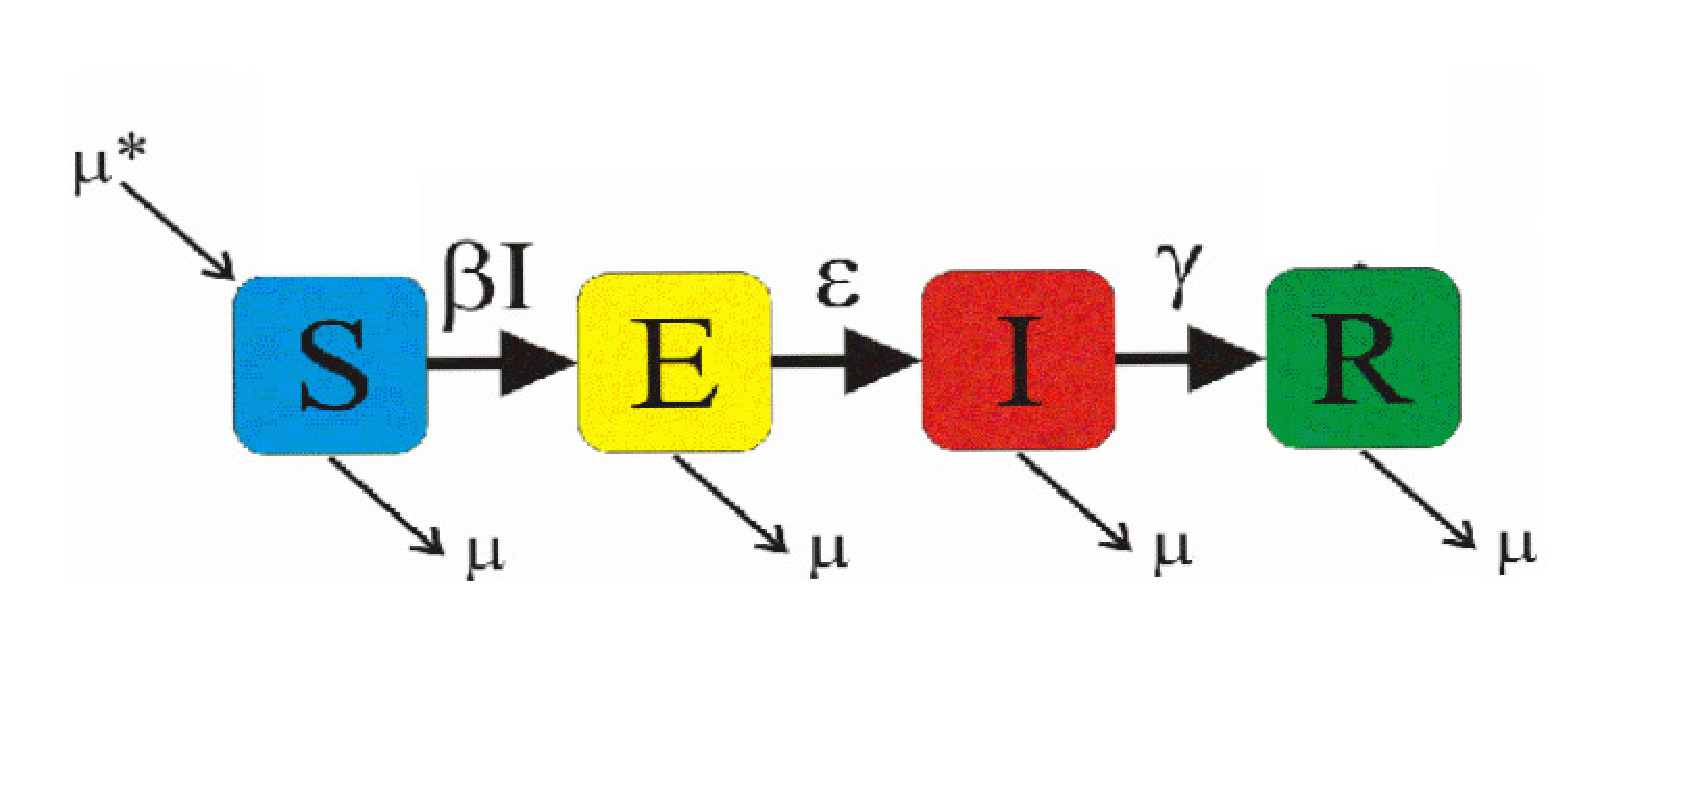
\includegraphics[scale=0.5]{figure/seirmodel} \protect\caption{SEIR model}
\label{fig:seirmodel} 
\end{figure}


In this model, the host population (N) is divided into four classes
: susceptible S(t), exposed E(t), infected I(t) and recovered R(t).
We have :

\textbf{$N(t)=S(t)+E(t)+I(t)+R(t)$ } 
\begin{itemize}
\item Class S(t) : contains the number of individuals not yet with the disease
at time t, or those susceptible to the disease. 
\item Class E(t) : contains the number of individuals who are in the exposed
or latent period of the disease. 
\item Class I(t) : contains the number of individuals who have been infected
with the disease and are capable of spreading the disease to those
in the susceptible category. 
\item Class R(t) : contains the number of individuals who have been infected
and then removed from the disease, either due to immunization or due
to death. Individuals of this class are not able to be infected again
or to transmit the disease infection to others. 
\end{itemize}
The conceptual descriptions of the model can be represented by a flow
diagram above. The flow diagram for the SEIR model uses arrows to
present the movement between the S and I classes, the E and I classes
and the I and R classes. Here, individuals are born susceptible, die
at a rate $\mu$, become infected with the force of infection $\lambda$
that is a function among the contact rate $\beta$, the number of
infected individual I and the population size N, infectious after
a latency period of an average duration of $1/\sigma$ and recover
at the rate $\gamma$.

The SEIR model is investigated by ordinary differential equations
(ODE) that are deterministic \cite{KeelingRohani2008}. The value
of variable states is only determined by parameters in the model and
by sets of previous states of these variables. Moreover, the epidemic
models are often proposed for one single population \cite{KeelingRohani2008}.
In the scope of this thesis, we propose a deterministic model for
many subpopulations in a metapopulation. The standard SEIR model (susceptible-exposed-infective-recovered)
has been strongly developed for the dynamics of directly infectious
disease \cite{Bolker1995}. For disease-based metapopulation models,
we give here a suit able new version of the SEIR equation that would
be as follows:

Consider a metapopulation of $n$ sub-populations. In a subpopulation
$i$ of size $N_{i}$, disease dynamics can be deterministically described
by the following set of differential equations \cite{Anderson&May1992}:

\begin{eqnarray}
\frac{dS_{i}}{dt} & = & \mu N_{i}-\lambda_{i}S_{i}-\mu S_{i}\label{eq:dS}\\
\frac{dE_{i}}{dt} & = & \lambda_{i}S_{i}-\mu E_{i}-\sigma E_{i}\\
\frac{dI_{i}}{dt} & = & \sigma E_{i}-\mu I_{i}-\gamma I_{i}\label{eq:infectieux}\\
\frac{dR_{i}}{dt} & = & \gamma I_{i}-\mu R_{i}\label{eq:dR}
\end{eqnarray}


where $S_{i}$, $E_{i}$, $I_{i}$ and $R_{i}$ are the numbers of
susceptible, exposed, infectious and recovered in this sub-population
$i$ respectively. Individuals are born susceptible, die at a rate
$\mu$, become infected with the force of infection $\lambda_{i}$,
infectious after a latency period of an average duration of $1/\sigma$
and recover at the rate $\gamma$. In a case the infectious contact
rate is constant, the equilibrium values of the variables $S$, $E$,
$I$ and $R$ can be expressed analytically (see late part). The force
of infection depends not only on the total population size $N_{i}$
and the number of infected $I_{i}$ in subpopulation $i$, but also
in other sub-populations \cite{KeelingRohani2008}:

\begin{equation}
\lambda_{i}=\sum_{j}\rho_{ij}\kappa_{j}\log\left[1-\sum_{k=1}^{M}\left(\frac{\left|I_{k,t}\right|}{N_{k}}\times c_{ik}\times\xi_{jk}\right)\right]\label{eq:force-1}
\end{equation}
where $c_{i,k}$ ($0\leqslant c_{ij}\leqslant1$) is the probability
that a susceptible individual native from $i$ being in contact with
another infected individual native from $k$ gets infected. $\xi_{jk}$
($0\leqslant\xi_{ij}\leqslant1$) refers to the probability that an
individual $y$ meeting $x$ in $C_{j}$ comes from $C_{k}$. $\kappa_{j}$
is the average number of contacts per unit of time a susceptible will
have when visiting subpopulation $j$. $\rho_{i,j}$ ($0\leqslant\rho_{ij}\leqslant1$)
is denoted as the probability that an individual from subpopulation
$i$ visits subpopulation $j$, of course, $\sum_{j=1}^{M}\rho_{ij}=1$.
See appendix for detail on the construction of this equation. We can
verify that in the limit case on one single subpopulation in the metapopulation
($i=j$ and $n=1$), we have:

\begin{equation}
\lambda_{i}=-\kappa_{i}\log(1-\frac{I_{i}}{N_{i}}\times c_{ii})
\end{equation}
Consider that the average number of contacts per unit of time $\kappa_{i}$
is seasonally forced \cite{Altizer2006} and seasonality is an annually
periodic function of time \cite{Grenfell1995}. As a result, for the
subpopulation $i$ :

\begin{equation}
\kappa_{i}(t)=\kappa_{i0}\left[1+\kappa_{i1}\cos\left(\frac{2\pi t}{T}+\varphi_{i}\right)\right]\label{eq:beta_i}
\end{equation}


where $t$ is the time, $\kappa_{i0}$ and $\kappa_{i1}$ are the
mean value and amplitude of the average contact rate $\kappa_{i}$
at which a susceptible will have when visiting subpopulation $i$
per unit of time, $T$ and $\varphi_{i}$ are the period and the phase
of the forcing. With the annual sinusoidal form of the average contact
rate, we really have the sinusoidally forced SEIR metapopulation model.

In detail, the deterministic model performs the same way for a given
set of initial conditions. It doesn't have randomness, dynamics, and
don't present dynamic of diseases in nature. Thus, stochastic models
have been proposed. A stochastic model is always more realistic than
a deterministic one. These models have stochastic and variable states
are not described by unique values, but by probability distributions.
It is why we will use the stochastic models to predict extinction
probability of disease in spatial context\cite{KeelingRohani2008}.


\subsubsection{Algorithms of stochastic simulation}

Stochastic simulation works on variables that both are random and
can be changed with certain probability. Today, these stochastic models
have been used widely in many domain because of some reasons as following
: before, in order to model chemically reacting systems, in simple
way, we solved a set of coupled ordinary differential equations (ODEs)
\cite{li2007stochastic} of deterministic approaches. Basically, these
approaches use the law of mass action that shows a simple relation
between reaction rate and molecular component concentrations. We start
with a given set of initial molecular concentrations, the law of mass
action permits us to see the component concentrations over time. The
states of a reaction are a homogeneous, free medium. The reaction
rate will be directly scaled with the concentrations of the elements.
Most systems can use the traditional deterministic approaches to simulate.
It is evident that many systems such as some biochemical systems consist
of random, discrete interactions between individual elements. However,
in the case, these systems becomes smaller and smaller, the traditional
deterministic models may not be accurate. It is the reason for that
the fluctuations of these systems can be simulated exactly by applying
stochastic models, particularly as well as the Stochastic Simulation
Algorithms (SSA) \cite{gillespie1976general,gillespie1977exact}.

The SSA uses Monte Carlo (MC) methods to study the time evolution
of the jump process. Because the basis feature of the Monte Carlo
simulation is insensitive to the dimensionality of the problem, and
the work grows linearly with the number of reaction channels in the
model. The SSA describes time-evolution statistically correct trajectories
of finite populations in continuous time by solving the corresponding
stochastic differential equations. Using the stochastic models can
solve three questions. (1) These models take account the discrete
character of the number of elements and the evidently random character
of collision among elements. (2) They coincide with the theories of
the dynamic and stochastic processes. (3) They are a good idea to
describe ``small systems'' and \textquotedbl{}instable systems''.
The main idea of the stochastic models is that element reactions are
essentially random processes. We don't know certainly how a reaction
occur at a moment. We also call it the process stochasticity. In particular,
in the process stochasticity, we talk about demographic and environmental
stochasticities in epidemic models. The demographic stochasticity
is strongly controlled by population size such as the birth and death
rates, contamination,etc. But, the environmental stochasticity is
just affected by environmental factors what we can not govern. Therefore,
there are many epidemic models that forcus on exploration of demographic
stochasticity. Demographic stochasticity is considered as fluctuation
in population processes that are based the random nature of events
at the level of the individual. Each event is related to one baseline
probability fixed, individuals are presented in differing fates due
to chance. In addition to the demographic stochasticity, the number
of infectious, susceptible, exposed and recovered individuals is now
required to be an integer. Modeling approaches that incorporate demographic
stochasticity are called event-driven methods. These methods require
explicit consideration of events. The first approach published by
Daniel T.Gillespie in 1976 \cite{gillespie1976general} is an exact
stochastic simulation approach for chemical kinetics. The Gillespie
stochastic simulation algorithm (SSA) has become the standard procedure
of the discrete-event modelling by taking proper value of the available
randomness in such a system. The methods modelling the event-driven
model demands explicit presentation of events. For the standard SEIR
model, we have to consider the nine events that can occur, each causing
the numbers in the relative groups to go up or down by one. Table
\ref{tab:stoch_event} lists all the events of the model, occurring
in subpopulation $i$ of a metapopulation:

\begin{table}[h]
\begin{tabular}{|c|c|c|}
\hline 
Events  & Rates  & Transitions \tabularnewline
\hline 
\hline 
birth  & $\mu N_{i}$  & $S_{i}\leftarrow S_{i}+1$ and $N_{i}\leftarrow N_{i}+1$\tabularnewline
\hline 
death of a susceptible  & $\mu S_{i}$  & $S_{i}\leftarrow S_{i}-1$ \tabularnewline
\hline 
death of an exposed  & $\mu E_{i}$  & \multicolumn{1}{c|}{$E_{i}\leftarrow E_{i}-1$ }\tabularnewline
\hline 
death of an infected  & $\mu I_{i}$  & $I_{i}\leftarrow I_{i}-1$ \tabularnewline
\hline 
death of an immune  & $\mu R_{i}$  & $I_{i}\leftarrow I_{i}-1$ \tabularnewline
\hline 
infection  & $\lambda_{i}S_{i}$  & $S_{i}\leftarrow S_{i}-1$ and $E_{i}\leftarrow E_{i}+1$ \tabularnewline
\hline 
becoming infectious  & $\sigma E_{i}$  & $E_{i}\leftarrow E_{i}-1$ and $I_{i}\leftarrow I_{i}+1$ \tabularnewline
\hline 
recovery  & $\gamma I_{i}$  & $I_{i}\leftarrow I_{i}-1$ and $R_{i}\leftarrow R_{i}+1$ \tabularnewline
\hline 
\end{tabular}

\protect\caption{Events of the stochastic version of the model of equations, occurring
in subpopulation $i$.}
\label{tab:stoch_event} 
\end{table}


To implement this SEIR stochastic model, there are many different
methods, thought most researchers often use the method of Gillespie
in 1977. Starting from the initial states, the stochastic simulation
algorithms simulate the trajectory in population processes by repeatedly
answering the following two questions and updating the states.
\begin{itemize}
\item When (time $\tau$) will the next reaction fire? 
\item Which (reaction channel index $\mu$) reaction will fire next? 
\end{itemize}
So the key parameters in the SSA model are $\tau$ and $\mu$. To
calculate these distributions, we set $a_{0}(x)=\sum_{j=1}^{M}a_{j}(x)$.
The time $\tau$, given $X(t)=x$, that the reaction will fire at
$t+\tau$, is the exponentially distributed random variable with mean
$\frac{1}{a_{0}(x)}$,

\begin{align*}
 & P(\tau=s)=a_{0}(x)exp(-a_{0}(x)s),\\
\end{align*}
\label{eqProbTau}

and the index $\mu$ is the integer random variable of that firing
reaction with probability :

\begin{align*}
 & P(\mu=j)=\frac{a_{j}(x)}{a_{0}(x)}\\
\end{align*}
\label{eqProbMu}

In each step, the SSA generates random numbers and calculates $\tau$
and $\mu$ according to the probability distribution \ref{eqProbTau}
and \ref{eqProbMu}. Below we will show some methods that simulate
exactly stochastic models. In this part, we will review the variant
formulations of Gillespie's stochastic simulation algorithm (SSA)
about the overview and the computational cost of each algorithm, then
approximate simulation methods, and finally hybrid and multi-scale
methods. We will also point out which algorithm that is most efficient,
which algorithm that we have used in this thesis.


\subsubsection{Exact stochastic simulation}

The key property for a discrete event simulation of a Markovian system
basically samples a time for the next event from this distribution
and selecting the reaction that occurs at that time. The Markovian
simulation methods have the basic steps of the widely used kinetic
Monte Carlo (KMC) method. First persons introduced the method (also
known as the KBL algorithm) are Young and Elcock in 1966 \cite{young1966monte}and
independently Lebowitz, Bortz and Kalos in 1975 \cite{bortz1975new}.
However, Gillespie really is the person who made kinetic Monte Carlo
popular in the chemical and biochemical domains, calling the algorithm
the Stochastic Simulation Algorithm (SSA) in his seminal articles
\cite{gillespie1976general,gillespie1977exact}. Below we will review
his two papers.
\begin{enumerate}
\item First reaction method (FRM) {[}GILLESPIE 1976{]} \cite{gillespie1977exact}:
The first reaction method was proposed by Gillespie in 1976. It models
demographic stochasticity in the more intuitive and slower way to
the deterministic model. The obtained result is \textquotedbl{}fluctuations
in population processes that arise from the random nature of events
at the level of the individual\textquotedbl{} \cite{KeelingRohani2008}.
The following pseudo-code provides a clean implementation of Gillespie's
first reaction method :


\begin{algorithm}[h]
0. Label all species $X_{1},...,X_{k}$.

1. Label all possible events $E_{1}$,...,$E_{n}$.

2. For each event determine the rate at which it occurs, $R_{1}$,...,$R_{n}$.

3. \textbf{While} $(t<t_{end}$ and $R_{N}=\sum_{v=1}^{n}R_{v}\neq0)$
\textbf{then}

4. \textbf{For} $ $$m=1,n$ \textbf{do}

5. Generate one random number $U(0,1)$ : $RAND_{m}$

6. At the event $m$ calculate the time until the next event is $\delta t_{m}=\frac{-1}{R_{m}}log(RAND_{m})$

7. \textbf{end for}

8. Find the event, $p$ , that happens first (has the smallest $\delta t$)

9. The time is now updated, $t\rightarrow\delta t_{p}$

10. Update $\{X_{i}\}$ following the event $p$.

11. Return to Step 3.

\protect\caption{Gillespie's first reaction method in 1976 - MONOPOPULATION}
\end{algorithm}



If supposing that generate one random number takes $C_{rand}$ time.
Then the FRM takes $nC_{rand}$ time per step. It is a big problem
for that Gillespie proposed a new improved algorithm in 1976. The
FRM has three main disadvantages : (1) generating random numbers is
relatively slow, (2) the FRM generates a cycle too many random numbers
in the case where the simulation time is big and the random number
generator will have tend on saturation when it generates too many
numbers, (3) the FRM is difficult for indexing the events to effectively
implement the update step.

\item Direct method (DM) {[}GILLESPIE 1977{]} \cite{gillespie1976general}:
The Direct Method was proposed by Gillespie in 1977. The main objective
is to present the stochastic simulation for chemically reacting systems.
The following pseudo-code of this method is :


\begin{algorithm}[h]
0. Label all species $X_{1},...,X_{k}$.

1. Label all possible events $E_{1}$,...,$E_{n}$.

2. For each event determine the rate at which it occurs, $R_{1}$,...,$R_{n}$.

3. \textbf{While} $(t<t_{end}$ and $R_{N}=\sum_{v=1}^{n}R_{v}\neq0)$
\textbf{then}

4. \textbf{For} $ $$m=1,n$ \textbf{do}

5. Calculate $R_{m}$ and $R_{m}=\sum_{v=1}^{m}R_{v}$

6. \textbf{end for}

7. Generate uniformly distributed random numbers $(r_{1},r_{2})$

8. Determine when $(\tau=ln(1/r_{1})/R_{N}$ and which $(min\{p|R_{p}\geq r_{2}R_{N}\})$
reaction will occur

9. Set $t=t+\tau$

10. Update $\{X_{i}\}$

11. Return to step 3

\protect\caption{Direct method of Gillespie in 1977 - MONOPOPULATION \cite{gillespie1976general}}
\end{algorithm}



We can find that on each step, the Direct Method has to generate two
random numbers. Supposing that generate one random number takes $C_{rand}$
time. Hence, on each step, the DM takes $(2C_{rand}+O(n))$ where
$O(n)$ is time to search the index $p$ of the next reaction channel.
For this reason, the DM is more efficient than the FRM.


The Gillespie algorithm plays an very important role and has become
a fundamental method in computational systems biology. Hence, many
efforts have been proposed to improve its efficiency. The key step
in the DM is to choose the next reaction channel to implement. This
step applies a linear search with a complexity $O(n)$ where $n$
is the number of occurred event in the system. Many methods have focused
on this step to improve and give more efficient formulations. For
example, Maksym in 1988 \cite{maksym1988fast} separated the set of
reactions into subsets with a complexity of $O(n^{1/2})$. In 1995,
Blue et al. \cite{blue1995faster} extended the division approach
of Maksym, where a $K-level$ method results in a search time proportional
to $n^{1/K}$. Then, in taking K to the limit, they applied a binary
tree structure and obtained the complexity $O(logR)$. Don't stop
improving, the Next Reaction Method (NRM) by Gibson and Bruck is more
known to the systems biology domain \cite{gibson2000efficient}.

\item Next Reaction Method (NRM) {[}GIBSON2000{]} \cite{gibson2000efficient}
In 2000, Gibson and Bruck successful transformed the algorithm FRM
into an equivalent but more efficient new structure. The Next Reaction
Method applies just a single random number per iteration. Moreover,
the initiation times of the reactions can be set as the firing times
of independent, unit rate Poisson processes with internal times given
by integrated propensity functions. It is evaluated steady faster
than the FRM and more efficient than DM in special cases as the system
includes many species and loosely coupled reaction channels. The NRM
is presented as follows :


\begin{algorithm}[h]
1. Initialize 
\begin{enumerate}
\item set initial numbers of species, set $t=0$, generate a dependency
graph $G$ 
\item calculate the propensity function $R{}_{j}(x)$, for all $j$ 
\item for each $j$, generate a putative time $\tau_{j}$ according to an
exponential distribution with parameter $R_{j}(x)$ 
\item store the $\tau_{j}$ values in an indexed priority queue $P$ 
\end{enumerate}
2. Let $\mu$ be the reaction whose putative time $\tau_{\mu}$ stored
in $P$ is least. Set $\tau=\tau_{\mu}$ 3. Update the states of the
species to reflect execution of reaction $\mu$. Set $t=\tau$ 4.
For each edge $(\mu,\alpha)$ in the dependency graph $G$ 
\begin{enumerate}
\item update $R_{\alpha}$ 
\item if $\alpha\neq\mu$, set $\tau_{\alpha}=R_{\alpha,old}/R_{\alpha,new}(\tau_{\alpha}-t)+t$ 
\item if $\alpha=\mu$, generate a random number $r$ and compute $\tau_{\alpha}$
according to an equation similar to Step 8 of the DM $\tau_{\alpha}=\frac{1}{R_{\alpha}(x)}log(\frac{1}{r})+t$ 
\item replace the old $R_{\alpha}$value in P with the new value. 
\end{enumerate}
Go to step 2.

\protect\caption{Next Reaction Method (NRM) {[}GIBSON2000{]}}
\end{algorithm}



The data structure presented in the NRM is a dependency graph. Because
a propensity function $R_{j}$ should be modified when a given reaction
is implemented. A node in the graph is correspondent to a reaction
channel. A directed edge of the reactions $A_{i}$ and $A_{j}$ points
out that the execution of $A_{i}$ really affects the molecules in
$A_{j}$. Due to the the dependency graph, in step 4, the number of
propensity functions recalculated is minimal.


In addition, the indexed priority queue is similar to a heap tree
in computer science. It is a tree that includes ordered pairs of the
form $(i,\tau_{i})$, where $i$ is both the reaction channel index
and the position in the tree, $\tau_{i}$ is the corresponding time
when the new $A_{i}$ reaction is expected to occur. In the tree,
the value $\tau$ of each parent is a smaller than that of its children.
The top node of the tree is always the minimum value of $\tau$ and
the order is only vertical. In each step, the nodes of the tree will
change its positions according to its value to get the new priority
queue.


In short, the NRM solved two additional optimizations : (1) by switching
to absolute time, Gibson and Bruck reduced the number of random numbers
needed in each step from two to one; (2) because of the use of a dependency
graph, the number of propensities needing to be recomputed for every
time step is minimum. In estimating the computation time of the NRM,
we find that, for every reaction channel, the time until that reaction
occurs is computed, maintained in an indexed priority queue, and efficiently
implemented as a binary heap. However, the cost for maintaining the
priority queue is relatively high. The time to select the next event
is done in constant time, but the time to update the propensities
is done in logarithmic time. Hence, the NRM is commonly used for systems
with many reaction channels and where relatively few propensities
change with each reaction. The disadvantage of the NRM is that diffusion
is added to the models and the reaction-diffusion master equation
is simulated, so systems arise. For such models, in 2004, Elf et al.
\cite{elf2004spontaneous} proposed a variant of the NRM that is called
the Next Subvolume Method (NSM). This method can be referred as a
clever association of the ideas of NRM and Maksym's method for intracellular
3D chemical reaction systems.

\item Compare the direct method (DM) to the next reaction method (NRM),
which algorithm is most efficient? We find that in the NRM, after
the executed first initial step, all sequent time steps only ask one
random number to be generated while the DM requests two. Even, the
search step for the index $\mu$ of the next reaction channel takes
$O(M)$ time for DM, but the corresponding task of updating the indexed
priority queue takes $log(M)$. It is the reason for that the NRM
is always evaluated more efficient for large scale problems. To evaluate
the real cost of two methods (NRM and DM) based on the total simulation
time, Yang Cao et al. \cite{Cao2004} made experiments for both formulations
of SSA on a 1.4 GHz Pentium IV Linux workstation. The problem used
in their experiments is a stochastic model of the heat shock response
of E. Coli \cite{kurata2001feedback}, which includes 28 variables
and 61 reactions. The experimental resultats pointed out that the
average simulation time for DM is larger than that for NRM due to
its data structure maintenance. In particular, for the loose coupling
system where the components (or elements) in a system are interconnected
and dependant on each other to the least extent practicable, NRM works
better than DM. Yang et al. found that three main factors that strongly
affect the CPU cost, are the costs, $C_{p}$ to calculate $M$ propensities,
$C_{a_{0}}$to calculate the sum of all propensity probabilities,
and $C_{s}$ to search for a event $\mu$. Hence, to reduce these
costs, Yang et al. \cite{Cao2004} suggested that a new optimization
called the Optimized Directed Method (ODM). They found that in a reaction
set of a system, some reactions fire much more frequently than others.
To reduce the search time $C_{s}$, they arranged the index of the
reaction ordering, placing the most frequently occurring events first
based on how often they fire, combined with a dependency graph, achieves
better results than the NRM for moderately large systems. Their optimized
direct method (ODM) gives a new search depth smaller than the original
method DM. The obtained result is that $C_{s}$ can be significantly
declined. In the next step to reduce the costs $C_{a_{0}}$ and $C_{p}$,
the authors used an idea from the method NRM. The ODM only recomputes
the propensities for those reaction channels affected by the last
reaction. Because of an extra cost used for accessing the dependency
graph, so this approach applies only to loose-coupling systems. In
conclusion, the obtained results of Yang et al. have shown that the
ODM is faster than NRM, in particular, unless the system is very nearly
uncoupled. This result broken the held belief for a long time that
NRM was the fastest.


Through this result, we can say that the efficiency of the ODM, currently
is evaluated to be the fastest known algorithm for stochastic simulation
for most biological problems. This method can be negatively impacted
by transient shifts in the frequency at which reactions occur, and
commonly used in biochemical reaction networks because of the inductive
and repressive nature of genetic regulation. Due to these shifts,
the ODM defeats the pre-simulation strategy employed within the ODM
to decrease the time complexity of the SSA's reaction selection step
and thus degrade performance. In order to decrease this degradation,
in 2005, McCollum et al. \cite{mccollum2006sorting} introduced the
sorting direct method (SDM) that improves on ODM. This method eliminates
the pre-simulations required by the ODM and permits the simulator
to adapt to sharp changes in reaction execution frequencies. The common
point of these two methods is to focus on the optimization of the
system instead of the method itself by reducing the average number
of operations required to obtain the index of the next reaction to
fire. This average number of operations is called the search depth
that is highly dependent on the biochemical system. For these two
methods, the search depth us $O(M)$. Besides, within the paper of
McCollum et al. \cite{mccollum2006sorting}, the authors also gave
a detailed overview of the difference in the implementation of DM,
NRM, ODM and SDM. In 2006, Li and Petzold introduced an alternative
formulation of the SSA, named the Logarithmic Direct Method (LDM).
In this method, the computational cost is independent of the ordering
of the reactions and no need for a pre-simulation. The LDM declined
the search depth to $O(logM)$, and pointed out the efficiency of
the logarithmic method.


Two years later, in 2008, a different approach is proposed by Hellander
\cite{hellander2008efficient} where the authors used the uniformity
and quasi-Monte Carlo to reduce the number of trajectories needed
to compute an approximation of the probability density function (PDF)
at the price of a higher cost per trajectory. Another is also found
to reduce the number of simulation in \cite{lecot2004quasi}. 

\end{enumerate}
A new search direction is very beneficial to generate ensembles of
trajectories in parallel. Because the parallelization of a single
trajectory is very hard. Apply clusters to implement SSA is proposed
by Li \cite{liStochKit}. Then, Li et al. continued executing SSA
on the graphics processing unit \cite{li2007stochastic,li2010efficient}.


\subsubsection{Approximate methods}

As mentioned above, the methods Direct, First Reaction and Next Reaction
are all exact stochastic approaches of the underlying ordinary differential
equations. Their advantage give us a really mathematically exact approach
to simulate time-to-event model (in condition that the definition
of the propensity functions accurately reflects the dynamics of the
system). But, their disadvantages are 1) noise in exact simulations
only affects the probabilities associated with fates of individuals
and the updating of each consecutive event is independent – there
is no assumption concerning environmental stochasticity; 2) these
exact solutions become too slow and impractical when any one transition
rate is large, when there is a big number of subpopulations or one
a big number of event in a metapopulation; because the exact algorithms
SSA must proceed one reaction at a time and take the task of explicitly
simulating each and every reaction event, hence they are much too
slow for most practical problems. It is the reason for that, approximate
models have been proposed instead of the exact stochastic methods.
The approximate approaches ask the question : \textquotedbl{}How many
times does each action channel fire in each subinterval?\textquotedbl{}

These approaches could be used in larger systems, and made much faster
than the exact methods. However, the exact structure of the Markov
chain is no longer simulated in the approximate approaches, hence
the validity of the approximations become a main issue. Now we will
show some mostly used approximate methods.
\begin{enumerate}
\item $\tau-leaping$ method Gillespie (2001) \cite{gillespie2001approximate}
has proposed a new method that decreases the simulation accuracy,
but speeds up the stochastic simulation. This is the explicit Poisson
$\tau-leap$ method known as an approximate method reduces the number
of iterations by treating transition rates as constant over time periods
for which this approximation leads to little error \cite{KeelingRohani2008}.
The $\tau-leap$ method applies a Poisson approximation to can “leap
over'' many fast reactions and approximate the stochastic behavior
of the system very well. The $\tau-leap$ method is described as follows
:


\begin{algorithm}
1. Let $\delta t$ be the time increment between steps, $\delta t$
is fixed as a constant. 2. Let $M_{T}(t)$ and $M_{R}(t)$ be the
number of transmission and recovery events by time $t$. 3. Setting
$\delta M_{i}=M_{i}(t+\delta t)-M_{i}(t)$ $i=T,R)$, then 
\begin{align*}
 & P(\delta M_{T}=1|X,Y) & = & \frac{\beta XY}{N}\delta t+o(\delta t)\\
 & P(\delta M_{R}=1|Y) & = & \gamma Y\delta t+o(\delta t)
\end{align*}
These two equations represent the transition probabilities for transmission
and recovery events occurring in the time interval $\delta t$. 4.
For small $\delta t$, the increments $\delta M_{i}$ are approximately
Poisson, such that: 
\begin{align*}
\delta M_{T} & \approx & Poisson(\frac{\beta XY}{N}\delta t)\\
\delta M_{R} & \approx & Poisson(\gamma Y\delta t)
\end{align*}
5. Updating the values of the variables : 
\begin{align*}
X(t+\delta t) & = & X(t)-\delta M_{T}+\delta M_{R}\\
Y(t+\delta t) & = & Y(t)+\delta M_{T}-\delta M_{R}
\end{align*}
6. Updating the time, $t=t+\delta t$. 7. Return to Step 4 \protect\caption{$\tau-leap$ method proposed by Gillespie (2001)\cite{KeelingRohani2008}}
\end{algorithm}



The main problem in the $\tau-leap$ method is relative to the value
of the time increment between steps, $\delta t$. How do we choose
the value fixed of $\delta t$? $\delta t$ must satisfy two conditions,
large enough so that many reaction events occur in that time and small
enough of the leap condition. The leap condition is pointed out that
\cite{cao2007adaptive}: For the current state $x$, the value of
$\delta t$ is asked to be small enought that the modification in
the state during $[t,t+\delta t]$ will be so small that no propensity
function will suffer an appreciable change in its value. Thus, the
key to the success of this technique is to choose a leap size large
enough to allow many reactions to occur during the leap (reducing
computation) and small enough that none of the propensity functions
will change significantly in value (causing an error). Cao et al.
\cite{cao2005avoiding} pointed also out a method to estimating the
largest value of $\delta t$, the expected change in each propensity
function during a leap be limited by $\epsilon a_{0}(x)$, where $\epsilon$
$(0<\epsilon\ll1)$ is the error control parameter. In short, the
best advantage of the $\tau-leap$ method is to speed up the stochastic
simulation for many ``not-too-stiff'' systems $-$i.e., systems
in which the difference between the characteristic time scales of
the fastest and slowest dynamical modes is not too large. However,
the number of firings of each reaction channels during a fixed time
step $\delta t$ is approximated as a Poisson random variable. This
Poisson variable can have arbitrarily large sample values. Hence,
there exists the possibility that this $\tau-leap$ method will cause
one or more reaction channels to fire so many times during $\delta t$
that number of reactants in each population will be became negative,
in particular in systems with multiple timescales (for short the stiff
systems). Due its obtained advantage, so this technique has continued
to mature, specially in the area of leap-size selection, through the
work of a variety of researchers : procedure for determining the maximum
leap size for a specified degree of accuracy \cite{gillespie2003improved};
a binomial leaping method developed independently Tian et al.\cite{tian2004binomial}
and Chatterjee et al. \cite{chatterjee2005binomial}; based on the
multinominal distribution by Pettigrew et al. in \cite{pettigrew2007multinomial};
the post-leap checks of Anderson \cite{Anderson&May1992}; and a further
work in this area can be expected. In detail for the binomial leaping
method, this method replaces the Poisson random variables with binomial
random variables, whose values are naturally bounded. However, the
disadvantage of this method appeared when the system is in the state
: there are multiple reactions with common consumed reactants, so
the issues of the binomial tau-leaping strategy have not yet been
fully resolved, and to write a general binomial tau-leaping program
that reliably handles all situations that could possibly arise, this
task would seem to be a very challenging task. It is the reason for
that, Yang et al. (2005) \cite{cao2005avoiding} is introduced a modified
Poisson tau-leaping procedure that also avoids negative populations
and these particular issues, but is easier to implement than the binomial
procedure. 

\end{enumerate}

\subsubsection{Hybrid and multiscale methods}
\begin{itemize}
\item Key word : Langevin equation, a Langevin equation is a stochastic
differential equation that could present the time advance of a subset
pf the degrees of freedom. In the epidemiology, the Langevin equations
are the equation that describe of the dynamics of the individuals
between the different compartments depends on the specific disease
considered. 
\end{itemize}
Here, we show an other kind of approximation methods that are based
on the validity of different approximations, and are the combination
of the deterministic equations and the Langevin equations for subsets
of the reactions, the chemical species or both. The results of these
methods have pointed out that the speedup obtained applying this hybrid
idea can be substantially. For example, Adalsteinsson et al. Combine
the deterministic and stochastic approaches in order to develop the
software package Biochemical Network Stochastic Simulator (BioNetS)
for efficiently and accurately simulating stochastic models of biochemical
networks in \cite{adalsteinsson2004biochemical}; the method that
applies chemical Langevin equations in \cite{gillespie2000chemical}
and in \cite{simpson2003frequency,simpson2004frequency}; Poisson-Runge-Kutta
methods \cite{burrage2004poisson}; multiscale algorithms like the
slow-scale stochastic simulation algorithm \cite{cao2005slow} and
use of the quasi-steady state assumption \cite{rao2003stochastic}.
Besides, there are many varieties of others, for exemple : Haseltine
and Rawlings \cite{haseltine2002approximate} associate deterministic
or Langevin equations for fast reactions with SSA for slow channels.
Saliz and Kazessis \cite{salis2005accurate} introduced a hybrid stochastic
method that divides the reaction set of the system into fast and slow
reaction subsets, applies a chemical Langevin equation for approximating
the fast reactions as a continuous Markov process, and has been used
successful to the simulation of the dynamics of a system based on
stochastic differential, ordinary differential, and master equations.
These methods are one part in the stock of current methods. To find
more information, readers can find detailed reviews in Turner et al.
\cite{turner2004stochastic} and Burrage et al. \cite{burrage2004poisson}.
In conclusion, so many researches have considered the approximate
methods as a strong solution to speed up simulations, however, to
exactly answer to question : where general biochemical modelers can
know when and when not to apply these methods, these techniques have
not matured yet. Inversely, exact stochastic simulation techniques
such as “exact method”, “direct method”,.. are inferior computational
methods, simulation time is large, but they remain effective, trusted,
and exact for simulating stochastic models in bio-informatics. It
is why, in my thesis, we use the exact method \textquotedbl{}Direct
Method\textquotedbl{} of Gillespie to modeling stochastic effects.


\section{DIZZYS : Description du modèle (ce qui corretspond au package R) }

The SEIR model have successful described hosts within a population
as Susceptible (the number of individuals not yet infected with the
disease), Exposed (the number of individuals who are infected with
the disease but not infectious),Infected (the number of individuals
who have been infected with the disease and are capable of spreading
the disease), and Recovered (the number of individuals who have successfully
cleared the infection). We ignore population demography-births, deaths,
and migration. So we have only three transitions: 

\begin{align*}
S\rightarrow E & E\rightarrow I & I\rightarrow R.\\
\end{align*}


It is obvious that the second and third of these are easier, so we
focus on the first transition in which the level of the infectious
disease influences strongly the disease transmission rate from a susceptible
individual into the infected class. If this first step doesn't occur,
all infected individuals can go to the recovered class. This first
transition plays an important role in studying fluctuation of disease.
Many researches have been tried to find the \textquotedbl{}infectious
period\textquotedbl{} (the amount of time spent in the infectious
class). They have found that for acute infections, the \textquotedbl{}infectious
period\textquotedbl{} is distributed around some mean values that
we can estimate from clinical data. To present enough properties of
the \textquotedbl{}infectious period\textquotedbl{} by formulations,
we have to depend upon three main factors of the disease transmission
from S to E : the prevalence of infecteds, the underlying population
contact structure, and the probability of transmission given contact.
For a directly transmitted disease, the key factor is the contact
between susceptible and infected individuals. Hence, in this section,
we will interpret the \textquotedbl{}infectious period\textquotedbl{}
in more detailed, and realistic contexts.

First of all, we define the force of infection, $\lambda$, which
is referred as the per capita rate at which susceptible individuals
contract the infection. The fact that $\lambda$ directly scales the
number of infectious individuals $I$. Moreover, for directly infectious
diseases, disease transmission demands contact between infecteds and
susceptibles. Hence, there are two proposed general possibilities
based on how we present the contact structure to change with population
size: $\lambda=\beta I/N$ applied when we want to mention frequency
dependent (or mass action) transmission, and $\lambda=\beta I$ applied
when we want to mention density dependent (or pseudo mass action)
transmission, where I is the number of infectious individuals, N is
the total population size (N=S+E+I+R), and $\beta$ is the product
of the contact rates and transmission probability. In the shape of
this thesis, we assume that the infection process is frequency-dependent,
meaning that the force of infection $\lambda$ is proportional to
a proportion of infected: $I/N$. Infection of susceptibles from one
population $i$ can be due to contacts with infected from the same
population $i$ or to contacts with infected from another population
$j$. In the next section, we will introduce a new mechanistic derivation
of the transmission term in more detailed, and realistic way.


\subsection{Infection force}

\textbf{Goal :} \\
 \textbf{Probabilistic derivation of multi-population epidemic model
with $\beta_{ijk}=-\kappa_{j}\log(1-c_{ik})$}

\textbf{Definition :}

During the small time interval $\delta t$, each native individual
of the city $i$ visits \textbf{a single} city $j$ (with probability
$\rho_{ij}$) and will meet \textbf{in average} $\kappa_{j}$ individuals
that come from all cities. 


\subsubsection{Notation}

\textbf{Notation :}

Here, we present list of sets and events describing the state of the
system at time $t$ : 
\begin{itemize}
\item $C_{i}$ is the set of all individuals born in subpopulation $i$. 
\item $V_{i,t}$ is the set of all individuals physically located in subpopulation
$i$ from time $t$ to time $t+\delta t$. This includes foreigners
traveling in subpopulation $i$ at time $t$, and all natives from
subpopulation $i$ which are not traveling abroad at time $t$. 
\item $S_{t},E_{t},I_{t},R_{t}$ are the sets of all individuals respectively
susceptible, exposed, infected and recovered at time $t$. Note that
these set include individuals from all subpopulations. 
\item $S_{i,t},E_{i,t},I_{i,t},R_{i,t}$ are the same sets, restricted to
natives of subpopulation $i$. So formally, $S_{i,t}=S_{t}\cap C_{i}$,
$E_{i,t}=E_{t}\cap C_{i}$, $I_{i,t}=I_{t}\cap C_{i}$, and $R_{i,t}=R_{t}\cap C_{i}$. 
\item $Transmit(y,x)$ is an event indicating that individual $x$ gets
infected by individual $y$ which was already infected 
\item $c_{i,k}$ is the probability that a susceptible individual native
from $i$ being in contact with another infected individual native
from $k$ gets infected. 
\item $\kappa_{j}$ is the average number of contacts per unit of time a
susceptible will have when visiting city $j$. 
\item $\xi_{jk}$ refers to the probability that an individual $y$ meeting
$x$ in $C_{j}$ comes from $C_{k}$. 
\item $\rho_{i,j}$, the probability that an individual from subpopulation
$i$ visits subpopulation $j$. Of course, $\sum_{j=1}^{M}\rho_{ij}=1$.
\end{itemize}
Note that : The coefficient $\kappa$ should also depend on $i$,
because an individual native from city $i$ meets more people in his
own city than abroad ($\kappa_{i,i}>\kappa_{i,j}$).


\subsubsection{The background}

\textbf{Let us write a probabilistic formulation of $\frac{dE_{i}}{dt}$:}
One general question is always posed \textquotedbl{}how does the population
of exposed individuals of subpopulation $i$ evolve ?\textquotedbl{}.
For the sake of simplicity, in the process of transmission of the
SEIR model, we focus on the incidence and we assume for now that the
latent period and the recovery rate, respectively $\mu=\sigma=0$.
Thus, we write a probabilistic formulation of $\frac{dE_{i}}{dt}$.
Assuming the time is discrete, we have $\frac{dE_{i}}{dt}\approx\mathbb{E}\left[E_{i,t+1}\setminus E_{i,t}\right]$.
Then,

\begin{eqnarray*}
\mathbb{E}\left[E_{i,t+1}\setminus E_{i,t}\right] & = & \mathbb{E}\left[E_{i,t+1}\cap S_{i,t}\right]\\
 & = & \sum_{x\in C_{i}}Pr\left[x\in E_{t+1}\wedge x\in S_{t}\right]\\
 & = & \sum_{x\in C_{i}}Pr\left[x\in S_{t}\right]*Pr\left[x\in E_{t+1}\mid x\in S_{t}\right]\\
 & = & Pr_{x\sim\mathcal{X}_{i}}\left[x\in E_{t+1}\mid x\in S_{t}\right]*\sum_{x\in C_{i}}Pr\left[x\in S_{t}\right]\\
 & = & |S_{i,t}|\times Pr_{x\sim\mathcal{X}_{i}}\left[x\in E_{t+1}\mid x\in S_{t}\right]
\end{eqnarray*}


Assume there are $M$ cities. An individual $x$ of the subpopulation
$i$ may be visiting another subpopulation, or staying in its own
subpopulation. Applying the law of total probabilities, we get:

\begin{eqnarray*}
Pr_{x\sim\mathcal{X}_{i}}\left[x\in E_{t+dt}\mid x\in S_{t}\right] & = & \sum_{j=1}^{M}Pr_{x\sim\mathcal{X}_{i}}\left[x\in E_{t+dt}\wedge x\in V_{j,t}\mid x\in S_{t}\right]\\
 & = & \sum_{j=1}^{M}Pr_{x\sim\mathcal{X}_{i}}\left[x\in E_{t+dt}\mid x\in S_{t}\wedge x\in V_{j,t}\right].Pr_{x\sim\mathcal{X}_{i}}\left[x\in V_{j,t}\right]\\
 &  & \sum_{j=1}^{M}Pr_{x\sim\mathcal{X}_{i}}\left[x\in E_{t+dt}\mid x\in S_{t}\wedge x\in V_{j,t}\right]\times\rho_{ij}
\end{eqnarray*}


Where $\rho_{i,j}=Pr_{x\sim\mathcal{X}_{i}}\left[x\in V_{j,t}\right]$,
the probability that an individual from subpopulation $i$ visits
subpopulation $j$. Of course, $\sum_{j=1}^{M}\rho_{ij}=1$.


\subsubsection{Study of case where agent $x$ native from subpopulation $i$ visits
subpopulation $j$}

Here, we look at the probability that a susceptible $x\sim\mathcal{X}_{i}$
visiting $j$ gets infected or not after $\delta t$ time steps. Let
$\mathcal{Y}$ be the uniform distribution over $V_{j,t}$. The correct
mathematical approach for this would be to assume that for each subpopulation
$k$, the number of people native from $k$ that we meet during $\delta t$
follows a Poisson process. So both the number of people we meet and
the number of infected people we meet during $\delta t$ should be
random variables.

In the approach described in \cite{KeelingRohani2008}, the authors
did not do this. They assumed that both the number of people we meet
and the number of infected people we meet \emph{are fixed} (otherwise
the maths they write would have been different). We will call this
the old interpretation of the infection force proposed by \textquotedbl{}Keeling
\& Rohani\textquotedbl{} (for short, OIIF) that we will present it
in the following parts.

We introduce an alternative approximation, where we assume that the
number $\kappa$ of people we meet during $\delta t$ is \emph{fixed},
but each of these people has \emph{some probability} to be infected.
This is an \emph{in-between interpretation}, easier than the Poisson
process maths, but better than the OIIF. We will call this the new
interpretation of the infection force (for short, NIIF).


\paragraph{1. The new interpretation: NIIF }

Agent $x$ meets \emph{exactly} $\kappa_{j}$ other individuals, and
each of these individuals has a probability $\frac{\left|I_{k,t}\right|}{N_{k}}$
of being infected, where $k$ is its native subpopulation. Let $y_{1}\ldots y_{\kappa_{j}}$
be the individuals that $x$ meets. We get: 

\begin{eqnarray*}
 &  & Pr_{x\sim\mathcal{X}_{i}}\left[x\in S_{t+\delta t}\mid x\in S_{t}\wedge x\in V_{j,t}\right]\\
 & = & Pr_{x\sim\mathcal{X}_{i},y_{1}\ldots,y_{\kappa_{j}}\sim\mathcal{Y}}\left[\bigwedge_{p=1}^{\kappa_{j}}\neg\left(y_{p}\in I_{t}\wedge Transmit(y_{p},x)\right)\mid x\in S_{t}\wedge x\in V_{j,t}\right]
\end{eqnarray*}


So we have: 
\begin{eqnarray*}
 &  & Pr_{x\sim\mathcal{X}_{i}}\left[x\in S_{t+\delta t}\mid x\in S_{t}\wedge x\in V_{j,t}\right]\\
 & = & Pr_{x\sim\mathcal{X}_{i},y\sim\mathcal{Y}}\left[\neg\left(y\in I_{t}\wedge Transmit(y,x)\right)\mid x\in S_{t}\wedge x\in V_{j,t}\right]^{\kappa_{j}\delta t}
\end{eqnarray*}


Moreover, we have: 
\begin{itemize}
\item the probability so that a susceptible individual $x$ is infected
by an infected individual $y$ : 
\end{itemize}
\begin{eqnarray*}
 &  & Pr_{x\sim\mathcal{X}_{i},y\sim\mathcal{Y}}\left[y\in I_{t}\wedge Transmit(y,x)\mid x\in S_{t}\wedge x\in V_{j,t}\right]\\
 & = & \sum_{k=1}^{M}Pr_{x\sim\mathcal{X}_{i},y\sim\mathcal{Y}}\left[y\in I_{t}\wedge Transmit(y,x)\mid x\in S_{t}\wedge x\in V_{j,t}\wedge y\in C_{k}\right].Pr_{y\sim\mathcal{Y}}\left(y\in C_{k}\right)\\
 & = & \sum_{k=1}^{M}\left\{ Pr_{x\sim\mathcal{X}_{i},y\sim\mathcal{X}_{k}}\left[y\in I_{t}\mid x\in S_{t}\wedge x\in V_{j,t}\right]\right.\\
 &  & \,\,\,\,\,\left.\times Pr_{x\sim\mathcal{X}_{i},y\sim\mathcal{X}_{k}}\left[Transmit(y,x)\mid y\in I_{t}\wedge x\in S_{t}\wedge x\in V_{j,t}\wedge y\in C_{k}\right]\times Pr_{y\sim\mathcal{Y}}\left(y\in C_{k}\right)\right\} \\
 & = & \sum_{k=1}^{M}\left(\frac{\left|I_{k,t}\right|}{N_{k}}\times c_{ik}\times\xi_{jk}\right)
\end{eqnarray*}


$\xi_{jk}=\frac{N_{k}\rho_{kj}}{\sum_{v=1}^{M}N_{v}\rho_{vj}}$ refers
to the probability that an individual $y$ meeting $x$ in $C_{j}$
comes from $C_{k}$. 
\begin{itemize}
\item hence, the probability so that a susceptible individual $x$ is not
infected by an infected individual $y$ : 
\end{itemize}
\[
1-\sum_{k=1}^{M}\left(\frac{\left|I_{k,t}\right|}{N_{k}}\times c_{ik}\times\xi_{jk}\right)
\]

\begin{itemize}
\item thereby, the probability so that a susceptible individual $x$ is
not infected after $\kappa_{j}$ contacts per unit time $\delta t$. 
\end{itemize}
\[
\left[1-\sum_{k=1}^{M}\left(\frac{\left|I_{k,t}\right|}{N_{k}}\times c_{ik}\times\xi_{jk}\right)\right]^{\kappa_{j}\delta t}
\]

\begin{itemize}
\item thus, the probability so that a susceptible individual $x$ becomes
infected after $\kappa_{j}$ contacts per unit time $\delta t$. 
\end{itemize}
\begin{eqnarray*}
Pr_{x\sim\mathcal{X}_{i}}\left[x\in E_{t+\delta t}\mid x\in S_{t}\wedge x\in V_{j,t}\right] & = & \left[1-\sum_{k=1}^{M}\left(\frac{\left|I_{k,t}\right|}{N_{k}}\times c_{ik}\times\xi_{jk}\right)\right]^{\kappa_{j}\delta t}
\end{eqnarray*}
We now apply the \emph{log} approximation which consists in approximating
$1-(1-u)^{v}$ by $v\log(1-u)$:

\begin{eqnarray*}
Pr_{x\sim\mathcal{X}_{i}}\left[x\in E_{t+\delta t}\mid x\in S_{t}\wedge x\in V_{j,t}\right] & = & -\kappa_{j}\delta t\log\left[1-\sum_{k=1}^{M}\left(\frac{\left|I_{k,t}\right|}{N_{k}}\times c_{ik}\times\xi_{jk}\right)\right]
\end{eqnarray*}


So, the transmission rate per susceptible individual is as follows:
\[
\frac{dPr_{x\sim\mathcal{X}_{i}}\left[x\in E_{t+dt}\mid x\in S_{t}\wedge x\in V_{j,t}\right]}{dt}\simeq-\kappa_{j}\log\left[1-\sum_{k=1}^{M}\left(\frac{\left|I_{k,t}\right|}{N_{k}}\times c_{ik}\times\xi_{jk}\right)\right]
\]


In fact, we use the parameter $\lambda$ to present this quantity,
and it is denoted as the \textquotedbl{}force of infection\textquotedbl{}
: x

If there is only one subpopulation $i$, then 
\[
\lambda_{i}=\kappa_{j}log(1-\frac{\left|I_{i}\right|}{N_{i}}\times c_{ii})
\]



\paragraph{2. The old Interpretation : OIIF \cite{KeelingRohani2008} }

Agent $x$ meets \emph{exactly} $\kappa_{j}\delta t\xi_{jk}\frac{\left|I_{k,t}\right|}{N_{k}}$
other infected individuals native from subpopulation $k$. Let $l_{k}=\kappa_{j}\delta t\xi_{jk}\frac{\left|I_{k,t}\right|}{N_{k}}$.
Let $y_{1}^{k}\ldots y_{l_{k}}^{k}$ be the infected individuals native
from $k$ that our individual $x$ meets between $t$ and $t+\delta t$.

We have the probability so that a susceptible individual $x$ is not
infected after having seen $l_{k}$ individuals between $t$ and $t+\delta t$:
\begin{eqnarray*}
 &  & Pr_{x\sim\mathcal{X}_{i}}\left[x\in S_{t+\delta t}\mid x\in S_{t}\wedge x\in V_{j,t}\right]\\
 & = & Pr_{x\sim\mathcal{X}_{i}}\left[\bigwedge_{\begin{array}{c}
k=1\ldots M\\
p=1\ldots l_{k}
\end{array}}\neg\left(Transmit(y_{p}^{k},x)\right)\mid x\in S_{t}\wedge x\in V_{j,t}\right]\\
 & = & \prod_{k=1}^{M}Pr_{x\sim\mathcal{X}_{i}}\left[\bigwedge_{p=1\ldots l_{k}}\neg\left(Transmit(y_{p}^{k},x)\right)\mid x\in S_{t}\wedge x\in V_{j,t}\right]\\
 & = & \prod_{k=1}^{M}\left(1-c_{ik}\right)^{\kappa_{j}\delta t\xi_{jk}\frac{\left|I_{k,t}\right|}{N_{k}}}
\end{eqnarray*}


Then, we plug this back into the previous formula, and we get: 
\begin{eqnarray*}
Pr_{x\sim\mathcal{X}_{i}}\left[x\in E_{t+\delta t}\mid x\in S_{t}\wedge x\in V_{j,t}\right] & = & 1-\prod_{k=1}^{M}\left(1-c_{ik}\right)^{\kappa_{j}\xi_{jk}\frac{\left|I_{k,t}\right|}{N_{k}}\delta t}
\end{eqnarray*}


The first order approximation of $1-\prod_{k=1}^{M}(1-c_{ik})^{v_{k}}$
is $\sum_{k=1}^{M}-v_{k}\log(1-c_{ik})$. Applying this approximation
here, we get:

\begin{eqnarray*}
Pr_{x\sim\mathcal{X}_{i}}\left[x\in E_{t+\delta t}\mid x\in S_{t}\wedge x\in V_{j,t}\right] & \simeq & \delta t\sum_{k=1}^{M}\left(-\kappa_{j}\xi_{jk}\frac{\left|I_{k,t}\right|}{N_{k}}\log\left(1-c_{ik}\right)\right)
\end{eqnarray*}


Define $\beta_{ijk}=-\kappa_{j}\log\left(1-c_{ik}\right)$, let $\delta t$
converge to zero, and we get: 
\[
\frac{dPr_{x\sim\mathcal{X}_{i}}\left[x\in E_{t+dt}\mid x\in S_{t}\wedge x\in V_{j,t}\right]}{dt}\simeq\sum_{k=1}^{M}\left(\xi_{jk}\frac{\left|I_{k,t}\right|}{N_{k}}\beta_{ijk}\right)
\]


If there is only one subpopulation $i$, then we fall back to the
formula of \cite{KeelingRohani2008}. We have : 
\[
\beta_{i}=-\kappa_{i}\log\left(1-c_{i}\right)
\]
\[
\frac{d}{dt}\mathbb{E}\left[\left|E_{i,t+dt}-E_{i,t}\right|\right]\simeq-\left|S_{i,t}\right|\left(\frac{\left|I_{i}\right|}{N_{i}}\beta_{i}\right)
\]
and the force of infection as follows : 
\[
\lambda_{i}=\beta_{i}\frac{\left|I_{i}\right|}{N_{i}}
\]



\paragraph{3. Final Formula }

We simply have to plug in the probability $\rho_{ij}$ that $i$ visits
$j$. We get, for the new interpretation NIIF:

\[
\frac{d}{dt}\mathbb{E}\left[\left|E_{i,t+dt}-E_{i,t}\right|\right]\simeq-\left|S_{i,t}\right|\sum_{j}\rho_{ij}\kappa_{j}\log\left[1-\sum_{k=1}^{M}\left(\frac{\left|I_{k,t}\right|}{N_{k}}\times c_{ik}\times\xi_{jk}\right)\right]
\]


And for the old interpretation OIIF \cite{KeelingRohani2008}:

\[
\frac{d}{dt}\mathbb{E}\left[\left|E_{i,t+dt}-E_{i,t}\right|\right]\simeq-\left|S_{i,t}\right|\sum_{j}\rho_{ij}\sum_{k=1}^{M}\left(\xi_{jk}\frac{\left|I_{k,t}\right|}{N_{k}}\beta_{ijk}\right)
\]


In conclusion, in this thesis, we use the interpretation NIIF to present
the infection force in meta-population. This interpretation shows
enough interactions between individuals in the same city, individuals
in different cities, and between cities in meta-population.


\subsection{The equilibrium state}

As mentioned above, we are interested in investigating the SEIR model
with demography. This model is an extension of the epidemic simple
SEIR model that allows for birth and death. Because, demographic processes
play an important role for exploring the longer-term persistence and
endemic dynamics of an infectious disease. In SEIR model with demography,
assuming that the time scale of disease propagation is fast enough
not to be affected by population births and deaths, the model is considered
in the case with a constant birth rate and a constant per-capita death
rate (that are independent of the population size). Now, we consider
a meta-population of many subpopulations. Each subpopulation is modelled
by a SEIR model with demography. Again, the ordinary differential
equations for a $subpopulation_{i}$ in a metapopulation is presented
as follows:

\begin{eqnarray}
\frac{dS_{i}}{dt} & = & \mu N_{i}-\lambda_{i}S_{i}-\mu S_{i}\\
\frac{dE_{i}}{dt} & = & \lambda_{i}S_{i}-\mu E_{i}-\sigma E_{i}\\
\frac{dI_{i}}{dt} & = & \sigma E_{i}-\mu I_{i}-\gamma I_{i}\\
\frac{dR_{i}}{dt} & = & \gamma I_{i}-\mu R_{i}
\end{eqnarray}


In simulation, we know that the equilibrium state allow a disease
to persist in a population for a long time, and the variables do not
change with time. So, an infectious disease in the $subpopulation_{i}$
is available in long term this system is at equilibrium. It means
that at which $\frac{dS_{i}}{dt}=\frac{dE_{i}}{dt}=\frac{dI{}_{i}}{dt}=\frac{dR{}_{i}}{dt}=0$
({*}). Thus, we let all ordinary differential equations in the system
be equal to zero, then calculate the values of the variables (now
denoted by $S_{i}^{*}$, $E_{i}^{*}$, $I_{i}^{*}$, and $R{}_{i}^{*}$)
that satisfy this condition ({*}). We have these values as follows:

\begin{eqnarray}
S_{i}^{*} & = & N_{i}\frac{(\gamma+\mu)(\sigma+\mu)}{\beta\sigma}\\
E_{i}^{*} & = & N_{i}\mu\left(\frac{1}{\sigma+\mu}-\frac{\gamma+\mu}{\beta\sigma}\right)\\
I_{i}^{*} & = & N_{i}\mu\frac{\beta\sigma-(\sigma+\mu)(\gamma+\mu)}{\beta(\sigma+\mu)(\gamma+\mu)}\\
R_{i}^{*} & = & N_{i}-S_{i}^{*}-E_{i}^{*}-I_{i}^{*}
\end{eqnarray}
Here, if we set $R_{0}=\frac{\beta\sigma}{(\gamma+\mu)(\sigma+\mu)}$,
so we have

\begin{eqnarray}
S_{i}^{*} & = & N_{i}\frac{1}{R_{0}}\\
E_{i}^{*} & = & N_{i}\frac{\mu\sigma}{R_{0}}\left(R_{0}-1\right)\\
I_{i}^{*} & = & N_{i}\frac{\mu}{\beta}(R_{0}-1)\\
R_{i}^{*} & = & N_{i}-S_{i}^{*}-E_{i}^{*}-I_{i}^{*}
\end{eqnarray}


One normal conditions for all population variables is that the equilibrium
values cannot be negative. Therefore, an infectious disease is available
in the $subpopulation_{i}$ if $R_{0}>1$. Now, the endemic equilibrium
in the system is given by $(S_{i}^{*},E_{i}^{*},I{}_{i}^{*},R{}_{i}^{*})$
= $(N_{i}\frac{1}{R_{0}}$, $N_{i}\frac{\mu\sigma}{R_{0}}\left(R_{0}-1\right)$,
$N_{i}\frac{\mu}{\beta}(R_{0}-1)$, $N_{i}(1-\frac{1}{R_{0}}-\frac{\mu\sigma}{R_{0}}\left(R_{0}-1\right)-\frac{\mu}{\beta}(R_{0}-1))$.


\subsection{DIZZYS : Description of package dizzys}

Stochastic and analytical methods are widely applied for the analysis
of epidemic models. Many simulation software as well as packages are
proposed to help scientists observe fluctuations of infectious diseases
over time. These tools simulate epidemic models either by dealing
with a set of ordinary differential equations (ODEs) or by applying
the stochastic simulation algorithm (SSA) of Gillespie. Simple epidemic
models work well on these software tools. However, the accuracy, the
simulation speed, and the complexity of models that the tools can
simulate are three main drawbacks that always prompt us not to stop
improving tools to increase efficient implementations available in
software tools. Moreover, rather than dynamics of infectious diseases,
predicting the potential spread of an infectious disease in a meta-population
is the most difficult problem for scientists. To give an exact prediction
about propagation of infectious diseases in a meta-population, we
need to make simulations in a complex meta-population with many interconnected
sub-populations where the meta-population takes into account many
factors about the pathogen, the climatic conditions and simultaneously
the interactions between sub-populations. Therefore, we introduce
the \textquotedbl{}dizzysNewInfec\textquotedbl{} package that allows
us to exactly simulate and accurately analyze dynamics of an infectious
disease in a meta-population of interconnected sub-populations by
using two basic and common disease models SIR and SEIR, and by implementing
the direct algorithm of Gillespie in 1977 and the adaptive tau leaping
to approximate the trajectory of a continuous-time stochastic process.
In addition, on the technical aspect, this package integrates C++
in R, we use C++ to build algorithms, and use R to show two-dimensional
and three-dimensional interfaces and use the available statistic functions
in R to analyze obtained results. Hence, dizzysNewInfec, it speeds
up simulations, it is very easy to install, to use and to show trajectories
of disease evolution over time in a meta-population of sub-populations.


\subsubsection{Introduction}

Fundamentally, Kermack-McKendrick gave the first epidemic model to
provide a mathematical description of the kinetic transmission of
an infectious disease in an unstructured sub-population. Due to this
model, today we have known well the SIR and SEIR deterministic epidemic
models. These two basic epidemic models are very popularly used by
scientists. The reactions in the system are modelled by a set of Ordinary
Differential Equations (ODEs) \cite{li2007stochastic}. The deterministic
method is the simplest to solve an epidemic model. The main idea of
this method is to solve a single differential equation per species
of the model. Basically, the deterministic method uses the law of
mass action that has applicability in many areas of science. In chemistry,
it is also called Fundamental Law of Chemical Kinetics (the study
of rates of chemical reactions), introduced by the Norwegian scientists
Cato M. Guldberg in 1864-1879 and Peter Waage. The law of mass action
shows a simple relation between reaction rate and molecular component
concentrations. For a set of initial molecular concentrations given,
the law of mass action permits us to see the component concentrations
over time. The states of a reaction are a homogeneous, free medium.
The reaction rate will be directly scaled with the concentrations
of the elements. Most systems can use the traditional deterministic
approaches to simulate. It is evident that many systems such as some
biochemical systems consist of random, discrete interactions between
individual elements. In fact, we have applied the deterministic model
in the epidemiology to solve epidemic models such as the SEIR and
SIR models. However, in the case, these systems become smaller and
smaller, the traditional deterministic models may not be accurate.
In addition, in the deterministic approach, the time evolution of
a reacting system is assumed that it is both continuous and deterministic.
But in fact, molecular population levels can change only by discrete
integer amounts. It is the reason for that this time evolution is
not both a continuous process and a discrete process. Indeed, the
deterministic approach is impossible to predict the exact molecular
population levels at some future times unless we can compute exactly
the precise positions and velocities of all molecules in the system.
It is the reason for that the fluctuations of these systems can be
simulated exactly by applying stochastic models via Stochastic Simulation
Algorithms (SSA) \cite{gillespie1976general,gillespie1977exact}.
The SSA uses Monte Carlo (MC) methods to study the time evolution
of the jump process. Because the basis feature of the Monte Carlo
simulation is insensitive to the dimensionality of the problem, and
the work grows linearly with the number of reaction channels in the
model. The SSA describes time-evolution statistically correct trajectories
of finite populations in continuous time by solving the corresponding
stochastic differential equations. Using the stochastic models can
solve three questions. (1) These models take account the discrete
character of the number of elements and the evidently random character
of collision among elements. (2) They coincide with the theories of
the dynamic and stochastic processes. (3) They are a good idea to
describe \textquotedbl{}small systems\textquotedbl{} and \textquotedbl{}unstable
systems\textquotedbl{}. The main idea of the stochastic models is
that element reactions are essentially random processes. We don't
know certainly how a reaction occurs at a moment. We also call it
the process stochasticity. Demographic stochasticity is considered
as fluctuation in population processes that is based the random nature
of events at the level of the individual. Each event is related to
one baseline probability fixed, individuals are presented in differing
fates due to chance. In addition to the demographic stochasticity,
the number of infectious, susceptible, exposed and recovered individuals
in a meta-population infected by an infectious disease is now required
to be an integer. Modeling approaches that incorporate demographic
stochasticity are called event-driven methods. These methods require
explicit consideration of events. The first approach published by
Daniel T.Gillespie in 1976 \cite{gillespie1976general} is an exact
stochastic simulation approach for chemical kinetics. The Gillespie
stochastic simulation algorithm (SSA) has become the standard procedure
of the discrete-event modelling by taking proper value of the available
randomness in such a system. The methods modelling the event-driven
model demands explicit presentation of events. Therefore, the \textquotedbl{}dizzysNewInfec\textquotedbl{}
package permits us to obtain the dynamics of the deterministic and
the stochastic dynamics of two basic epidemic models SIR and SEIR.
We use the exact algorithm of Gillespie in 1977 and the \textquotedbl{}adaptive
tau-leaping\textquotedbl{} algorithm in the package. With these two
algorithms, each has its private advantages and its private disadvantages.
For the exact algorithm, it gives us a really exact approach of simulating
population-based time-to-event through two steps with many iterations
of 1) searching the time of next event by an exponentially distributed
function and 2) searching the nature of next event. Each single event
in the Gillespie's solution is explicitly simulated, so this exact
simulation becomes exceedingly slow and impractical in systems where
the transition rate grows large over time. Hence, approximate models
are born instead of the Gillespie's solution, they are concerned with
larger transition rates and with increasing simulation speed while
still maintaining reasonable accuracy. The \textquotedbl{}adaptive
tau-leaping\textquotedbl{} algorithm known as an approximate method
reduces the number of iterations by treating transition rates as constant
over time periods for which this approximation leads to little error
\cite{Cao2007}.

The SEIR epidemic model used in our package have successful described
hosts within a population as Susceptible (the number of individuals
not yet infected with the disease), Exposed (the number of individuals
who are infected with the disease but not infectious), Infected (the
number of individuals who have been infected with the disease and
are capable of spreading the disease), and Recovered (the number of
individuals who have successfully cleared the infection). We ignore
population demography-births, deaths, and migration. So we have only
three transitions: 
\begin{equation}
S\rightarrow E,E\rightarrow I,I\rightarrow R.
\end{equation}
It is obvious that the second and third of these transitions are easier,
so we focus on the first transition in which the level of the infectious
disease influences strongly the disease transmission rate from a susceptible
individual into the infected class. If this first step doesn't occur,
all infected individuals can go to the recovered class. This first
transition plays an important role in studying fluctuation of disease.
Many researches have been tried to find the \textquotedbl{}infectious
period\textquotedbl{} (the amount of time spent in the infectious
class). They have found that for acute infections, the \textquotedbl{}infectious
period\textquotedbl{} is distributed around some mean values that
we can estimate from clinical data. To present enough properties of
the \textquotedbl{}infectious period\textquotedbl{} by formulations,
we have to depend upon three main factors of the disease transmission
from S to E : the prevalence of infecteds, the underlying population
contact structure, and the probability of transmission given contact.
For a directly transmitted disease, the key factor is the contact
between susceptible and infected individuals. Hence, in this package
\textquotedbl{}dizzysNewInfe\textquotedbl{}, we interpret the \textquotedbl{}infectious
period\textquotedbl{} in more detailed, and realistic contexts. We
introduce a new formula of the probabilistic derivation of multipopulation
epidemic model called NIIF. We study the case where agent $x$ native
from subpopulation $i$ visits sub-population $j$. In a meta-population
of sub-populations, during a small interval of time $\delta t$, each
native individual of the sub-population $i$ visits one single sub-population
$j$ (with probability $\rho_{ij}$) and will see on average $K_{j}$.
These individuals come from all sub-populations. This is absolutely
a new interpretation about the infection between individuals and the
propagation of disease between sub-population. In previous research
described in {[}keeling2011{]}, the authors always assumed that both
the number of people we meet and the number of infected people we
meet are fixed. This assumption simplifies the relations between individuals
and between sub-populations. It's the reason for that the formula
of the infection force did not present clearly the complex connections
between individuals and between sub-populations in a meta-population.
In our interpretation, we assume that for each sub-population $k$,
the number of people native from $k$ that we meet during $\delta t$
follows a Poisson process. So both the number of people we meet and
the number of infected people we meet during $\delta t$ should be
random variables.

In short, the \textbf{dizzysNewInfec} package implements both the
exact solution and the approximate solution for the SIR and SEIR models.
The package installs well the new interpretation of the infection
force NIIF for SIR and SEIR meta-population models by integrating
the R package and the C++ implementation. We can choose one of these
two solutions to simulate when the number of sub-populations in a
meta-population increases. Using C++ to perform the algorithms, and
R to create interfaces makes the \textbf{dizzysNewInfec} package much
faster and much easy to use than any pure R package.


\subsubsection{Methods}

In this section, first we will talk about the deterministic and stochastic
SEIR models. Then, we will present transformation the SEIR model into
the SIR model through the usage of the two algorithms. We hope that
the models and the algorithms should be well understood before obtaining
simulation results.


\paragraph{1. Deterministic SEIR model: }

To describe infectious diseases in a in a spatial context, we consider
a meta-population of n sub-populations. In sub-population $i$ of
size $N_{i}$, disease dynamics can be deterministically described
by the following set of differential equations:

\begin{eqnarray}
\frac{dS_{i}}{dt} & = & \mu N_{i}-\lambda_{i}S_{i}-\mu S_{i}\label{eq:dS-1}\\
\frac{dE_{i}}{dt} & = & \lambda_{i}S_{i}-\mu E_{i}-\sigma E_{i}\\
\frac{dI_{i}}{dt} & = & \sigma E_{i}-\mu I_{i}-\gamma I_{i}\label{eq:infectieux-1}\\
\frac{dR_{i}}{dt} & = & \gamma I_{i}-\mu R_{i}\label{eq:dR-1}
\end{eqnarray}


where $S_{i}$, $E_{i}$, $I_{i}$ et $R_{i}$ are respectively the
numbers of susceptible, exposed, infectious and recovered in this
sub-population $i$. Individuals are born susceptible and die at a
rate $\mu$, become infected with the force of infection $\lambda_{i}$,
infectious after a latency period of an average duration of $1/\sigma$
and recover at the rate $\gamma$. In case the infectious contact
rate is constant, the equilibrium values of the variables $S$, $E$,
$I$ and $R$ can be expressed analytically. The force of infection
depends not only on the total population size $N_{i}$ and the number
of infected $I_{i}$ in subpopulation $i$, but also in other sub-populations
:

\[
\lambda_{i}=\sum_{j}\rho_{ij}\kappa_{j}\log\left[1-\sum_{k=1}^{M}\left(\frac{\left|I_{k,t}\right|}{N_{k}}\times c_{ik}\times\xi_{jk}\right)\right]
\]


where $\rho_{i,j}$ the probability that an individual from sub-population
$i$ visits sub-population $j$. $\kappa_{j}$ is the average number
of contacts per unit of time a susceptible will have when visiting
city. $c_{i,k}$ is the probability that a susceptible individual
native from $i$ being in contact with another infected individual
native from $k$. $\xi_{jk}$ refers to the probability that an individual
$y$ meeting $x$ in $C_{j}$ comes from $C_{k}$. See appendix for
detail on the construction of this equation. We can verify that in
the limit case on one single subpopulation in the metapopulation ($i=j$
and $n=1$), we have :

\begin{equation}
\lambda_{i}=-\kappa_{i}\log(1-\frac{I_{i}}{N_{i}}\times c_{ii})
\end{equation}


In the case, we consider that the contact number $K_{i}$ is seasonally
forced {[}Altizer2006{]}: 
\begin{equation}
K_{i}(t)=K_{i0}\left[1+K_{i1}\cos\left(\frac{2\pi t}{T}+\varphi_{i}\right)\right]\label{eq:beta_i-1}
\end{equation}
where $K_{i0}$ and $K_{i1}$ are the mean value and amplitude of
the contact number and $T$ and $\varphi_{i}$ are the period and
the phase of the forcing.


\paragraph{2. Stochastic models}



The stochastic model is built by depending upon the deterministic
model. More detailed, this stochastic model relies on chance variation
in risks of exposure, disease, and other factors. It is referred as
an individual-level modeling, because every individual plays an important
role in the model, so this stochastic model can consider well most
small population size that the deterministic model can not do. To
implement this SEIR stochastic model, there are many different methods.
The first method \textquotedbl{}First Reaction Method\textquotedbl{}
is born in 1976 by Gillespie. Then, according to this first method
and these two key factors of demographic stochasticity models (event,
randomness), many scientists have improved the first method, and created
many better algorithms for stochastic simulations. There are two main
types of methods, exact methods and approximative methods. The typical
approach in exact methods most practitioners use, is the algorithm
\textquotedbl{}Direct Method\textquotedbl{} of Gillespie(1977) improved
from the first approach \textquotedbl{}First Reaction Method\textquotedbl{},
and in approximative methods, is the \textquotedbl{}tau-leaping\textquotedbl{}
method. For the Direct Method (Gillespie 1977), the first step estimates
the time until the next event, by accumulating the rates of all possible
events. Then, by transforming event rates into probabilities, the
method randomly selects one of these events. The time and numbers
in each class are then updated according to which event is chosen.
We repeat this process to iterate model through time. For the \textquotedbl{}tau-leaping\textquotedbl{}
method, the main crux is the use of Poisson random variables to approximate
the number of occurrences of each type of reaction event during a
carefully selected time period, $\tau$ . According to these two types
of algorithms, the common point is both methods use continuous-time
Markov process for which the transition rates are constants, isn't
a function of time. The future state of the process, is only conditional
on the present state, but independent of the past. However, for the
exact algorithm, its advantage give us a really exact approach to
simulate time-to-event model. This process is repeated to iterate
the mode. GibsonBruck(2000) \cite{KeelingRohani2008} modified the
first reaction method and created the Next Reaction method that substantially
more challenging to program but is significantly faster than even
the method when there are a large number of different event types.
The Direct, First Reaction and Next Reaction methods are all exact
stochastic approaches of the underlying ordinary differential equations.
But, its disadvantages are 1) noise in exact simulations only affects
the probabilities associated with fates of individuals and the updating
of each consecutive event is independent – there is no assumption
concerning environmental stochasticity; 2) these exact solutions become
too slow and impractical when any one transition rate is large, when
there is a big number of sub-populations or one a big number of event
in a meta-population. It is the reason for that, approximate models
have been proposed instead of the exact stochastic methods. Gillespie
(2001) has proposed a new method that decreases the simulation accuracy,
but increases simulation speed. This is the \textquotedbl{}tau-leap
method\textquotedbl{} known as an approximate method reduces the number
of iterations by treating transition rates as constant over time periods
for which this approximation leads to little error {[}KeelingRohani2008{]}
as mentioned above. However, when we use the \textquotedbl{}tau-leap
method\textquotedbl{}, there is a possibility, the number of individual
in each class can become negative. According to Keeling2008\cite{KeelingRohani2008},
the authors compared these methods together, they pointed out that
when the population size increases, the simulation time of the three
methods (First Reaction, Direct Method, tau -leap ) is almost augmented.
The simulation time of the method \textquotedbl{}First Method\textquotedbl{}
is maximum, it means that this is the slowest method, but the simulation
time of the method \textquotedbl{}tau-leap\textquotedbl{} is minimum
or the fastest. In the shape of my package, we use the direct method
to exactly estimate spread of diseases in meta-population. Because
the direct method is one exact approach and its simulation time isn't
too slow and too fast. We use the approximate method to speed up simulations
in the case where there are many sub-populations in a meta-population.


\subparagraph{a. Direct method}

Based on the differential equations above, we give a stochastic version
of this model. We use for that a population-based time-to-next-event
model based on Gillespie's algorithm {[}Daniel.T.Gillespie1977{]}.
Table \ref{tab:stoch_ev} lists all the events of the model, occurring
in subpopulation $i$.

\begin{table}[htpb]
\begin{centering}
\caption{\label{tab:stoch_ev}Events of the stochastic version of the model
of equations, occuring in subpopulation $i$.}

\par\end{centering}

\centering{}% %
\begin{tabular}{lcc}
\textbf{Events}  & \textbf{Rates}  & \textbf{Transitions }\tabularnewline
\textbf{birth}  & $\mu N_{i}$  & $S_{i}\leftarrow S_{i}+1$ and $N_{i}\leftarrow N_{i}+1$ \tabularnewline
\textbf{death of a susceptible}  & \textbf{$\mu S_{i}$}  & \textbf{$S_{i}\leftarrow S_{i}-1$ }\tabularnewline
\textbf{death of an exposed}  & \textbf{$\mu E_{i}$}  & \textbf{$E_{i}\leftarrow E_{i}-1$ }\tabularnewline
\textbf{death of an infected}  & \textbf{$\mu I_{i}$}  & \textbf{$I_{i}\leftarrow I_{i}-1$ }\tabularnewline
\textbf{death of an immune}  & \textbf{$\mu R_{i}$}  & \textbf{$I_{i}\leftarrow I_{i}-1$ }\tabularnewline
\textbf{infection}  & \textbf{$\lambda_{i}S_{i}$}  & \textbf{$S_{i}\leftarrow S_{i}-1$ }and\textbf{ $E_{i}\leftarrow E_{i}+1$ }\tabularnewline
\textbf{becoming infectious}  & \textbf{$\sigma E_{i}$}  & \textbf{$E_{i}\leftarrow E_{i}-1$ }and\textbf{ $I_{i}\leftarrow I_{i}+1$ }\tabularnewline
\textbf{recovery}  & \textbf{$\gamma I_{i}$}  & \textbf{$I_{i}\leftarrow I_{i}-1$ }and\textbf{ $R_{i}\leftarrow R_{i}+1$ }\tabularnewline
 &  & \tabularnewline
\end{tabular}
\end{table}


To apply the Direct Method in a meta-population of n sub-populations,
we know that at a moment $t$, there are only one single event fired
in one single sub-population during one time unit $tstep$. Hence,
we improve the Direct Method for one single population by adding a
random number to calculate chance which sub-population to fire. Starting
from the initial states, the stochastic simulation algorithms simulate
the trajectory in population processes by repeatedly answering the
following three big questions and updating the states.
\begin{itemize}
\item When (time) will the next event occur? 
\item Which subpopulation where the event will occur next? 
\item Which event in the subpopulation will occur next? 
\end{itemize}
Although, it is a small improvement in the original Direct Method,
however it turns back much more benefits for a meta-population, it
well presents the interactions between subpopulations in the metapopulation.


\subparagraph{b. Adaptive tau-leaping algorithm}

In this step, we provide basic concepts for the adaptive tau-leaping
algorithm by using the detailed description of Cao {[}Cao2007{]}.

For the Markov process at time t, to describe a metapopulation of
n subpopulations, we have:

\textbf{state set:} X(t)

$X(t):=[S_{1}(t),...,S_{n}(t),E_{1}(t),...,E_{n}(t),I_{1}(t),...,I_{n}(t),R_{1}(t),...,R_{n}(t)]$

each variables of $X(t)$ is defined on the non-negative integers.

\textbf{set of allowable transitions:} ${\triangle_{j}}$, for each
allowable transition, $j$, we define a rate $\lambda_{j}$, by using
a function independent on t but dependent on the current state $X(t)$,
to calculate transition rates given the state $(\lambda(X))$ through
the deterministic model, and a vector of $n$ integers, $\triangle_{j}:=[\triangle_{j,1},...,\triangle_{j,n}]$,
that reflects the change in state if this transition were followed:
$X(t)+\triangle_{j}$.

\textbf{time process: }modeling on a time-homogeneous process.

\textbf{operation:} with the SEIR model, the package simulates a trajectory
from time $0$ to a stopping time $tmax$. Based on the description
of Cao and al. in 2007, a good time period of length $\tau$ is during
which all transition rates remain approximately constant and all $n$
state variables remain greater than zero with probability$\thicksim1$.
Then, by using the Poisson-dustributed number of transitions, that
should have occurred during this period: $X(t+\tau)\approx X(t)+\sum_{j}y_{j}\triangle_{j}$
where $y_{j}\thicksim Poisson(\tau\lambda_{j})$. To successfully
apply this algorithm, we need to know that, transition rates frequently
change and in balancing efficiency with accuracy when selecting these
time periods to leap over.

In short, in the package \textquotedbl{}dizzysNewInfec\textquotedbl{}
we have build successfully the Direct method and \textquotedbl{}tau-leap
method\textquotedbl{} for a meta-population. In the particular case,
there is one single sub-population, the Direct Method and \textquotedbl{}tau-leap\textquotedbl{}
method for a meta-population are similar to the original methods.


\paragraph{3. Transformation SEIR model into SIR model:}

The deterministic SEIR model with one subpopulation by exploiting
the 'seir' function in the package.


\subsubsection{Example}

\%\%\%\%\%\%\%\%\%\%


\subsubsection{Comparison between the packages ``dizzysNewInfec'' and other packages}


\paragraph{a. Between the packages ``dizzysNewInfec'' and ``GillespieSSA''
\cite{pineda2008gillespiessa}}
\begin{itemize}
\item Introduction ``GillespieSSA''
\item the possibility of GillespieSSA and of Dizzys
\item Fastness
\item Conclusion
\end{itemize}
\%\%\%\%\%\%\%\%\%\%\%\%\%\%


\paragraph{b. Between the packages ``dizzysNewInfec'' and ``adaptivetau''
\cite{johnson2011adaptivetau}}
\begin{itemize}
\item comparaison avec ce qui existe déjà en termes de (1) possibilité (ce
que l’on peut faire) et de (2) rapidité. En gros il y a un compromis
entre flexibilité et rapidité
\item à comparer avec “adaptivetau” et “GillespieSSA”. Voir aussi les autres
outils qu’il existe
\item Kullback-Leibler Divergence or Kolmogorov–Smirnov test to compare
the simulation results.
\item Package ‘EpiDynamics’
\end{itemize}

\paragraph{c. Between the packages ``dizzysNewInfec'' and ``EpiDynamics''
\cite{baquero2014EpiDynamics}}

%%%%%%

\%\%\%\%\%\%

\%\%\%


\section{Relation structure/dynamique spatiale et persistence }

C’est ce que tu es en train d’explorer pour le moment. Plusieurs questions
à explorer. Chaque question constitue un sous-chapitre. A toi de développer
et structurer cette partie plus en détails.


\section{Contrôle par reinforcement learning: }
\begin{itemize}
\item comment utiliser ton simulateur pour faire du reinforcement learning.
Partie qui reste à développer. 
\end{itemize}

\section{Conclusion et discussion générales.}

Commence donc à écrire certaines parties dès que tu peux (un peu chaque
semaine et de plus en plus au fur et à fur que le temps avance). Pense
aussi à bien faire la bibliographie (il faut que tu sois incollable
sur le sujet). Les nouveau login et mot de passe de Bibliovie (http://bibliovie.inist.fr)
sont 15SCBUMR5290 et 4NX9E5. Ou, on peux utiliser l'account de Giang
à UPMC selon les conseil de la site : http://www.jubil.upmc.fr/fr/ressources\_en\_ligne2/mode\_acces\_ressources.html.

 \bibliographystyle{plain}
\bibliography{biblio/bibManuscrit}

\end{document}
